\documentclass[1p]{elsarticle_modified}
%\bibliographystyle{elsarticle-num}

%\usepackage[colorlinks]{hyperref}
%\usepackage{abbrmath_seonhwa} %\Abb, \Ascr, \Acal ,\Abf, \Afrak
\usepackage{amsfonts}
\usepackage{amssymb}
\usepackage{amsmath}
\usepackage{amsthm}
\usepackage{scalefnt}
\usepackage{amsbsy}
\usepackage{kotex}
\usepackage{caption}
\usepackage{subfig}
\usepackage{color}
\usepackage{graphicx}
\usepackage{xcolor} %% white, black, red, green, blue, cyan, magenta, yellow
\usepackage{float}
\usepackage{setspace}
\usepackage{hyperref}

\usepackage{tikz}
\usetikzlibrary{arrows}

\usepackage{multirow}
\usepackage{array} % fixed length table
\usepackage{hhline}

%%%%%%%%%%%%%%%%%%%%%
\makeatletter
\renewcommand*\env@matrix[1][\arraystretch]{%
	\edef\arraystretch{#1}%
	\hskip -\arraycolsep
	\let\@ifnextchar\new@ifnextchar
	\array{*\c@MaxMatrixCols c}}
\makeatother %https://tex.stackexchange.com/questions/14071/how-can-i-increase-the-line-spacing-in-a-matrix
%%%%%%%%%%%%%%%

\usepackage[normalem]{ulem}

\newcommand{\msout}[1]{\ifmmode\text{\sout{\ensuremath{#1}}}\else\sout{#1}\fi}
%SOURCE: \msout is \stkout macro in https://tex.stackexchange.com/questions/20609/strikeout-in-math-mode

\newcommand{\cancel}[1]{
	\ifmmode
	{\color{red}\msout{#1}}
	\else
	{\color{red}\sout{#1}}
	\fi
}

\newcommand{\add}[1]{
	{\color{blue}\uwave{#1}}
}

\newcommand{\replace}[2]{
	\ifmmode
	{\color{red}\msout{#1}}{\color{blue}\uwave{#2}}
	\else
	{\color{red}\sout{#1}}{\color{blue}\uwave{#2}}
	\fi
}

\newcommand{\Sol}{\mathcal{S}} %segment
\newcommand{\D}{D} %diagram
\newcommand{\A}{\mathcal{A}} %arc


%%%%%%%%%%%%%%%%%%%%%%%%%%%%%5 test

\def\sl{\operatorname{\textup{SL}}(2,\Cbb)}
\def\psl{\operatorname{\textup{PSL}}(2,\Cbb)}
\def\quan{\mkern 1mu \triangleright \mkern 1mu}

\theoremstyle{definition}
\newtheorem{thm}{Theorem}[section]
\newtheorem{prop}[thm]{Proposition}
\newtheorem{lem}[thm]{Lemma}
\newtheorem{ques}[thm]{Question}
\newtheorem{cor}[thm]{Corollary}
\newtheorem{defn}[thm]{Definition}
\newtheorem{exam}[thm]{Example}
\newtheorem{rmk}[thm]{Remark}
\newtheorem{alg}[thm]{Algorithm}

\newcommand{\I}{\sqrt{-1}}
\begin{document}

%\begin{frontmatter}
%
%\title{Boundary parabolic representations of knots up to 8 crossings}
%
%%% Group authors per affiliation:
%\author{Yunhi Cho} 
%\address{Department of Mathematics, University of Seoul, Seoul, Korea}
%\ead{yhcho@uos.ac.kr}
%
%
%\author{Seonhwa Kim} %\fnref{s_kim}}
%\address{Center for Geometry and Physics, Institute for Basic Science, Pohang, 37673, Korea}
%\ead{ryeona17@ibs.re.kr}
%
%\author{Hyuk Kim}
%\address{Department of Mathematical Sciences, Seoul National University, Seoul 08826, Korea}
%\ead{hyukkim@snu.ac.kr}
%
%\author{Seokbeom Yoon}
%\address{Department of Mathematical Sciences, Seoul National University, Seoul, 08826,  Korea}
%\ead{sbyoon15@snu.ac.kr}
%
%\begin{abstract}
%We find all boundary parabolic representation of knots up to 8 crossings.
%
%\end{abstract}
%\begin{keyword}
%    \MSC[2010] 57M25 
%\end{keyword}
%
%\end{frontmatter}

%\linenumbers
%\tableofcontents
%
\newcommand\colored[1]{\textcolor{white}{\rule[-0.35ex]{0.8em}{1.4ex}}\kern-0.8em\color{red} #1}%
%\newcommand\colored[1]{\textcolor{white}{ #1}\kern-2.17ex	\textcolor{white}{ #1}\kern-1.81ex	\textcolor{white}{ #1}\kern-2.15ex\color{red}#1	}

{\Large $\underline{12a_{0709}~(K12a_{0709})}$}

\setlength{\tabcolsep}{10pt}
\renewcommand{\arraystretch}{1.6}
\vspace{1cm}\begin{tabular}{m{100pt}>{\centering\arraybackslash}m{274pt}}
\multirow{5}{120pt}{
	\centering
	\includegraphics[width=112pt]{../../../GIT/diagram.site/Diagrams/png/1510_12a_0709.png}\\
\ \ \ A knot diagram\footnotemark}&
\allowdisplaybreaks
\textbf{Linearized knot diagam} \\
\cline{2-2}
 &
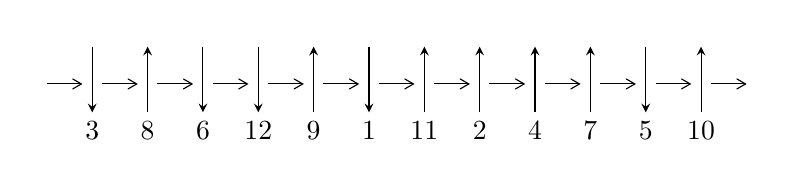
\begin{tikzpicture}[x=20pt, y=17pt]
	% nodes
	\node (C0) at (0, 0) {};
	\node (C1) at (1, 0) {};
	\node (C1U) at (1, +1) {};
	\node (C1D) at (1, -1) {3};

	\node (C2) at (2, 0) {};
	\node (C2U) at (2, +1) {};
	\node (C2D) at (2, -1) {8};

	\node (C3) at (3, 0) {};
	\node (C3U) at (3, +1) {};
	\node (C3D) at (3, -1) {6};

	\node (C4) at (4, 0) {};
	\node (C4U) at (4, +1) {};
	\node (C4D) at (4, -1) {12};

	\node (C5) at (5, 0) {};
	\node (C5U) at (5, +1) {};
	\node (C5D) at (5, -1) {9};

	\node (C6) at (6, 0) {};
	\node (C6U) at (6, +1) {};
	\node (C6D) at (6, -1) {1};

	\node (C7) at (7, 0) {};
	\node (C7U) at (7, +1) {};
	\node (C7D) at (7, -1) {11};

	\node (C8) at (8, 0) {};
	\node (C8U) at (8, +1) {};
	\node (C8D) at (8, -1) {2};

	\node (C9) at (9, 0) {};
	\node (C9U) at (9, +1) {};
	\node (C9D) at (9, -1) {4};

	\node (C10) at (10, 0) {};
	\node (C10U) at (10, +1) {};
	\node (C10D) at (10, -1) {7};

	\node (C11) at (11, 0) {};
	\node (C11U) at (11, +1) {};
	\node (C11D) at (11, -1) {5};

	\node (C12) at (12, 0) {};
	\node (C12U) at (12, +1) {};
	\node (C12D) at (12, -1) {10};
	\node (C13) at (13, 0) {};

	% arrows
	\draw[->,>={angle 60}]
	(C0) edge (C1) (C1) edge (C2) (C2) edge (C3) (C3) edge (C4) (C4) edge (C5) (C5) edge (C6) (C6) edge (C7) (C7) edge (C8) (C8) edge (C9) (C9) edge (C10) (C10) edge (C11) (C11) edge (C12) (C12) edge (C13) ;	\draw[->,>=stealth]
	(C1U) edge (C1D) (C2D) edge (C2U) (C3U) edge (C3D) (C4U) edge (C4D) (C5D) edge (C5U) (C6U) edge (C6D) (C7D) edge (C7U) (C8D) edge (C8U) (C9D) edge (C9U) (C10D) edge (C10U) (C11U) edge (C11D) (C12D) edge (C12U) ;
	\end{tikzpicture} \\
\hhline{~~} \\& 
\textbf{Solving Sequence} \\ \cline{2-2} 
 &
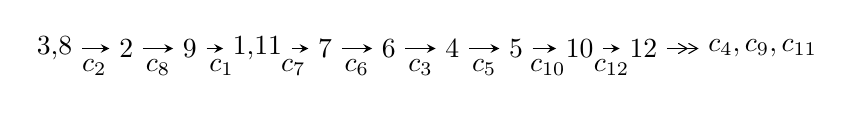
\begin{tikzpicture}[x=23pt, y=7pt]
	% node
	\node (A0) at (-1/8, 0) {3,8};
	\node (A1) at (1, 0) {2};
	\node (A2) at (2, 0) {9};
	\node (A3) at (49/16, 0) {1,11};
	\node (A4) at (33/8, 0) {7};
	\node (A5) at (41/8, 0) {6};
	\node (A6) at (49/8, 0) {4};
	\node (A7) at (57/8, 0) {5};
	\node (A8) at (65/8, 0) {10};
	\node (A9) at (73/8, 0) {12};
	\node (C1) at (1/2, -1) {$c_{2}$};
	\node (C2) at (3/2, -1) {$c_{8}$};
	\node (C3) at (5/2, -1) {$c_{1}$};
	\node (C4) at (29/8, -1) {$c_{7}$};
	\node (C5) at (37/8, -1) {$c_{6}$};
	\node (C6) at (45/8, -1) {$c_{3}$};
	\node (C7) at (53/8, -1) {$c_{5}$};
	\node (C8) at (61/8, -1) {$c_{10}$};
	\node (C9) at (69/8, -1) {$c_{12}$};
	\node (A10) at (11, 0) {$c_{4},c_{9},c_{11}$};

	% edge
	\draw[->,>=stealth]	
	(A0) edge (A1) (A1) edge (A2) (A2) edge (A3) (A3) edge (A4) (A4) edge (A5) (A5) edge (A6) (A6) edge (A7) (A7) edge (A8) (A8) edge (A9) ;
	\draw[->>,>={angle 60}]	
	(A9) edge (A10);
\end{tikzpicture} \\ 

\end{tabular} \\

\footnotetext{
The image of knot diagram is generated by the software ``\textbf{Draw programme}" developed by Andrew Bartholomew(\url{http://www.layer8.co.uk/maths/draw/index.htm\#Running-draw}), where we modified some parts for our purpose(\url{https://github.com/CATsTAILs/LinksPainter}).
}\phantom \\ \newline 
\centering \textbf{Ideals for irreducible components\footnotemark of $X_{\text{par}}$} 
 
\begin{align*}
I^u_{1}&=\langle 
-4.12238\times10^{643} u^{173}-1.44902\times10^{644} u^{172}+\cdots+5.70533\times10^{643} b+4.68445\times10^{646},\\
\phantom{I^u_{1}}&\phantom{= \langle  }-4.22603\times10^{644} u^{173}-1.65272\times10^{645} u^{172}+\cdots+2.45329\times10^{645} a+8.91828\times10^{647},\\
\phantom{I^u_{1}}&\phantom{= \langle  }u^{174}+4 u^{173}+\cdots+860 u-1849\rangle \\
I^u_{2}&=\langle 
-5.49547\times10^{30} u^{44}+1.24545\times10^{32} u^{43}+\cdots+1.16778\times10^{31} b-1.49742\times10^{32},\\
\phantom{I^u_{2}}&\phantom{= \langle  }8.02764\times10^{31} u^{44}-2.04849\times10^{32} u^{43}+\cdots+1.16778\times10^{31} a-7.33963\times10^{31},\;u^{45}-3 u^{44}+\cdots+5 u-1\rangle \\
\\
\end{align*}
\raggedright * 2 irreducible components of $\dim_{\mathbb{C}}=0$, with total 219 representations.\\
\footnotetext{All coefficients of polynomials are rational numbers. But the coefficients are sometimes approximated in decimal forms when there is not enough margin.}
\newpage
\renewcommand{\arraystretch}{1}
\centering \section*{I. $I^u_{1}= \langle -4.12\times10^{643} u^{173}-1.45\times10^{644} u^{172}+\cdots+5.71\times10^{643} b+4.68\times10^{646},\;-4.23\times10^{644} u^{173}-1.65\times10^{645} u^{172}+\cdots+2.45\times10^{645} a+8.92\times10^{647},\;u^{174}+4 u^{173}+\cdots+860 u-1849 \rangle$}
\flushleft \textbf{(i) Arc colorings}\\
\begin{tabular}{m{7pt} m{180pt} m{7pt} m{180pt} }
\flushright $a_{3}=$&$\begin{pmatrix}1\\0\end{pmatrix}$ \\
\flushright $a_{8}=$&$\begin{pmatrix}0\\u\end{pmatrix}$ \\
\flushright $a_{2}=$&$\begin{pmatrix}1\\u^2\end{pmatrix}$ \\
\flushright $a_{9}=$&$\begin{pmatrix}u\\u^3+u\end{pmatrix}$ \\
\flushright $a_{1}=$&$\begin{pmatrix}u^2+1\\u^2\end{pmatrix}$ \\
\flushright $a_{11}=$&$\begin{pmatrix}0.172259 u^{173}+0.673674 u^{172}+\cdots+253.690 u-363.523\\0.722548 u^{173}+2.53976 u^{172}+\cdots-53.2667 u-821.065\end{pmatrix}$ \\
\flushright $a_{7}=$&$\begin{pmatrix}0.422411 u^{173}+1.39381 u^{172}+\cdots-302.931 u-346.299\\0.615721 u^{173}+2.61270 u^{172}+\cdots+1393.76 u-1631.60\end{pmatrix}$ \\
\flushright $a_{6}=$&$\begin{pmatrix}-0.0184136 u^{173}+0.0945368 u^{172}+\cdots+652.785 u-378.198\\0.202712 u^{173}+1.00516 u^{172}+\cdots+981.542 u-855.900\end{pmatrix}$ \\
\flushright $a_{4}=$&$\begin{pmatrix}0.193671 u^{173}+0.530332 u^{172}+\cdots-488.877 u-18.5190\\0.111537 u^{173}+0.537748 u^{172}+\cdots+289.103 u-383.316\end{pmatrix}$ \\
\flushright $a_{5}=$&$\begin{pmatrix}0.307311 u^{173}+1.07846 u^{172}+\cdots-26.6558 u-386.220\\0.566995 u^{173}+2.38261 u^{172}+\cdots+1178.68 u-1453.70\end{pmatrix}$ \\
\flushright $a_{10}=$&$\begin{pmatrix}-0.204957 u^{173}-0.619119 u^{172}+\cdots+448.630 u-11.9952\\0.00105037 u^{173}+0.0260070 u^{172}+\cdots+66.3987 u-59.8984\end{pmatrix}$ \\
\flushright $a_{12}=$&$\begin{pmatrix}0.0524607 u^{173}+0.336201 u^{172}+\cdots+567.209 u-430.018\\0.303407 u^{173}+1.43438 u^{172}+\cdots+1226.11 u-1130.46\end{pmatrix}$\\&\end{tabular}
\flushleft \textbf{(ii) Obstruction class $= -1$}\\~\\
\flushleft \textbf{(iii) Cusp Shapes $= -0.188361 u^{173}-1.56403 u^{172}+\cdots-2713.89 u+2013.65$}\\~\\
\newpage\renewcommand{\arraystretch}{1}
\flushleft \textbf{(iv) u-Polynomials at the component}\newline \\
\begin{tabular}{m{50pt}|m{274pt}}
Crossings & \hspace{64pt}u-Polynomials at each crossing \\
\hline $$\begin{aligned}c_{1}\end{aligned}$$&$\begin{aligned}
&u^{174}+78 u^{173}+\cdots+38633006 u+3418801
\end{aligned}$\\
\hline $$\begin{aligned}c_{2},c_{8}\end{aligned}$$&$\begin{aligned}
&u^{174}+4 u^{173}+\cdots+860 u-1849
\end{aligned}$\\
\hline $$\begin{aligned}c_{3}\end{aligned}$$&$\begin{aligned}
&81(81 u^{174}-2520 u^{173}+\cdots+1289568 u-74248)
\end{aligned}$\\
\hline $$\begin{aligned}c_{4},c_{11}\end{aligned}$$&$\begin{aligned}
&9(9 u^{174}+30 u^{173}+\cdots+188726 u-372821)
\end{aligned}$\\
\hline $$\begin{aligned}c_{5}\end{aligned}$$&$\begin{aligned}
&u^{174}-5 u^{173}+\cdots+9544707 u+120123
\end{aligned}$\\
\hline $$\begin{aligned}c_{6}\end{aligned}$$&$\begin{aligned}
&u^{174}+2 u^{173}+\cdots+4585039248 u-391773717
\end{aligned}$\\
\hline $$\begin{aligned}c_{7},c_{10}\end{aligned}$$&$\begin{aligned}
&9(9 u^{174}+12 u^{173}+\cdots-2.70063\times10^{7} u-1.08127\times10^{7})
\end{aligned}$\\
\hline $$\begin{aligned}c_{9}\end{aligned}$$&$\begin{aligned}
&u^{174}+u^{173}+\cdots-62865261 u+31013523
\end{aligned}$\\
\hline $$\begin{aligned}c_{12}\end{aligned}$$&$\begin{aligned}
&u^{174}+13 u^{173}+\cdots+3315627075 u+351801391
\end{aligned}$\\
\hline
\end{tabular}\\~\\
\newpage\renewcommand{\arraystretch}{1}
\flushleft \textbf{(v) Riley Polynomials at the component}\newline \\
\begin{tabular}{m{50pt}|m{274pt}}
Crossings & \hspace{64pt}Riley Polynomials at each crossing \\
\hline $$\begin{aligned}c_{1}\end{aligned}$$&$\begin{aligned}
&y^{174}+50 y^{173}+\cdots-1038422793520482 y+11688200277601
\end{aligned}$\\
\hline $$\begin{aligned}c_{2},c_{8}\end{aligned}$$&$\begin{aligned}
&y^{174}+78 y^{173}+\cdots+38633006 y+3418801
\end{aligned}$\\
\hline $$\begin{aligned}c_{3}\end{aligned}$$&$\begin{aligned}
&6561\\
&\cdot(6561 y^{174}-457002 y^{173}+\cdots+161502458592 y+5512765504)
\end{aligned}$\\
\hline $$\begin{aligned}c_{4},c_{11}\end{aligned}$$&$\begin{aligned}
&81(81 y^{174}+10620 y^{173}+\cdots+5.06180\times10^{12} y+1.38995\times10^{11})
\end{aligned}$\\
\hline $$\begin{aligned}c_{5}\end{aligned}$$&$\begin{aligned}
&y^{174}-21 y^{173}+\cdots+1241320767183 y+14429535129
\end{aligned}$\\
\hline $$\begin{aligned}c_{6}\end{aligned}$$&$\begin{aligned}
&y^{174}+52 y^{173}+\cdots+2.28\times10^{19} y+1.53\times10^{17}
\end{aligned}$\\
\hline $$\begin{aligned}c_{7},c_{10}\end{aligned}$$&$\begin{aligned}
&81\\
&\cdot(81 y^{174}-8172 y^{173}+\cdots+749524157872730 y+116915411184049)
\end{aligned}$\\
\hline $$\begin{aligned}c_{9}\end{aligned}$$&$\begin{aligned}
&y^{174}-25 y^{173}+\cdots-29120310824125347 y+961838608871529
\end{aligned}$\\
\hline $$\begin{aligned}c_{12}\end{aligned}$$&$\begin{aligned}
&y^{174}-57 y^{173}+\cdots-3.54\times10^{18} y+1.24\times10^{17}
\end{aligned}$\\
\hline
\end{tabular}\\~\\
\newpage\flushleft \textbf{(vi) Complex Volumes and Cusp Shapes}
$$\begin{array}{c|c|c}  
\text{Solutions to }I^u_{1}& \I (\text{vol} + \sqrt{-1}CS) & \text{Cusp shape}\\
 \hline 
\begin{aligned}
u &= -0.788449 + 0.612244 I \\
a &= \phantom{-}1.01781 + 1.02674 I \\
b &= \phantom{-}2.04982 - 0.76639 I\end{aligned}
 & \phantom{-}10.83900 + 1.99487 I & \phantom{-0.000000 } 0 \\ \hline\begin{aligned}
u &= -0.788449 - 0.612244 I \\
a &= \phantom{-}1.01781 - 1.02674 I \\
b &= \phantom{-}2.04982 + 0.76639 I\end{aligned}
 & \phantom{-}10.83900 - 1.99487 I & \phantom{-0.000000 } 0 \\ \hline\begin{aligned}
u &= \phantom{-}0.416392 + 0.912492 I \\
a &= -0.709660 + 0.446722 I \\
b &= -1.43573 + 0.63145 I\end{aligned}
 & -0.96633 + 2.24854 I & \phantom{-0.000000 } 0 \\ \hline\begin{aligned}
u &= \phantom{-}0.416392 - 0.912492 I \\
a &= -0.709660 - 0.446722 I \\
b &= -1.43573 - 0.63145 I\end{aligned}
 & -0.96633 - 2.24854 I & \phantom{-0.000000 } 0 \\ \hline\begin{aligned}
u &= \phantom{-}0.879645 + 0.469234 I \\
a &= -0.969777 + 1.013240 I \\
b &= -1.66320 - 0.81580 I\end{aligned}
 & \phantom{-}5.45213 - 8.38927 I & \phantom{-0.000000 } 0 \\ \hline\begin{aligned}
u &= \phantom{-}0.879645 - 0.469234 I \\
a &= -0.969777 - 1.013240 I \\
b &= -1.66320 + 0.81580 I\end{aligned}
 & \phantom{-}5.45213 + 8.38927 I & \phantom{-0.000000 } 0 \\ \hline\begin{aligned}
u &= -0.830633 + 0.547297 I \\
a &= \phantom{-}1.128490 + 0.494286 I \\
b &= \phantom{-}1.75016 - 0.96820 I\end{aligned}
 & \phantom{-}5.98006 - 4.36530 I & \phantom{-0.000000 } 0 \\ \hline\begin{aligned}
u &= -0.830633 - 0.547297 I \\
a &= \phantom{-}1.128490 - 0.494286 I \\
b &= \phantom{-}1.75016 + 0.96820 I\end{aligned}
 & \phantom{-}5.98006 + 4.36530 I & \phantom{-0.000000 } 0 \\ \hline\begin{aligned}
u &= -0.205645 + 0.985061 I \\
a &= -0.192720 + 1.021700 I \\
b &= -1.37963 + 0.31976 I\end{aligned}
 & -0.464505 + 1.123620 I & \phantom{-0.000000 } 0 \\ \hline\begin{aligned}
u &= -0.205645 - 0.985061 I \\
a &= -0.192720 - 1.021700 I \\
b &= -1.37963 - 0.31976 I\end{aligned}
 & -0.464505 - 1.123620 I & \phantom{-0.000000 } 0\\
 \hline 
 \end{array}$$\newpage$$\begin{array}{c|c|c}  
\text{Solutions to }I^u_{1}& \I (\text{vol} + \sqrt{-1}CS) & \text{Cusp shape}\\
 \hline 
\begin{aligned}
u &= \phantom{-}0.509642 + 0.868302 I \\
a &= -2.52058 - 1.09872 I \\
b &= -0.57422 - 2.65776 I\end{aligned}
 & \phantom{-}1.66281 + 2.05945 I & \phantom{-0.000000 } 0 \\ \hline\begin{aligned}
u &= \phantom{-}0.509642 - 0.868302 I \\
a &= -2.52058 + 1.09872 I \\
b &= -0.57422 + 2.65776 I\end{aligned}
 & \phantom{-}1.66281 - 2.05945 I & \phantom{-0.000000 } 0 \\ \hline\begin{aligned}
u &= \phantom{-}0.847140 + 0.550886 I \\
a &= -0.715555 - 1.063980 I \\
b &= -0.156423 - 0.621752 I\end{aligned}
 & \phantom{-}5.23383 - 8.16565 I & \phantom{-0.000000 } 0 \\ \hline\begin{aligned}
u &= \phantom{-}0.847140 - 0.550886 I \\
a &= -0.715555 + 1.063980 I \\
b &= -0.156423 + 0.621752 I\end{aligned}
 & \phantom{-}5.23383 + 8.16565 I & \phantom{-0.000000 } 0 \\ \hline\begin{aligned}
u &= -0.857862 + 0.488258 I \\
a &= -0.793497 - 1.022840 I \\
b &= -1.41627 + 0.86799 I\end{aligned}
 & \phantom{-}4.48914 + 3.16789 I & \phantom{-0.000000 } 0 \\ \hline\begin{aligned}
u &= -0.857862 - 0.488258 I \\
a &= -0.793497 + 1.022840 I \\
b &= -1.41627 - 0.86799 I\end{aligned}
 & \phantom{-}4.48914 - 3.16789 I & \phantom{-0.000000 } 0 \\ \hline\begin{aligned}
u &= -0.553950 + 0.811931 I \\
a &= \phantom{-}1.036070 + 0.516539 I \\
b &= \phantom{-}2.70747 - 0.97654 I\end{aligned}
 & \phantom{-}4.71428 - 4.00424 I & \phantom{-0.000000 } 0 \\ \hline\begin{aligned}
u &= -0.553950 - 0.811931 I \\
a &= \phantom{-}1.036070 - 0.516539 I \\
b &= \phantom{-}2.70747 + 0.97654 I\end{aligned}
 & \phantom{-}4.71428 + 4.00424 I & \phantom{-0.000000 } 0 \\ \hline\begin{aligned}
u &= \phantom{-}0.444757 + 0.876054 I \\
a &= \phantom{-}0.055749 - 1.041920 I \\
b &= -0.624114 + 0.797198 I\end{aligned}
 & -0.91368 + 1.26387 I & \phantom{-0.000000 } 0 \\ \hline\begin{aligned}
u &= \phantom{-}0.444757 - 0.876054 I \\
a &= \phantom{-}0.055749 + 1.041920 I \\
b &= -0.624114 - 0.797198 I\end{aligned}
 & -0.91368 - 1.26387 I & \phantom{-0.000000 } 0\\
 \hline 
 \end{array}$$\newpage$$\begin{array}{c|c|c}  
\text{Solutions to }I^u_{1}& \I (\text{vol} + \sqrt{-1}CS) & \text{Cusp shape}\\
 \hline 
\begin{aligned}
u &= -0.582917 + 0.786807 I \\
a &= \phantom{-}0.664644 - 0.051473 I \\
b &= \phantom{-}0.695866 + 0.908138 I\end{aligned}
 & \phantom{-}2.79384 + 2.54567 I & \phantom{-0.000000 } 0 \\ \hline\begin{aligned}
u &= -0.582917 - 0.786807 I \\
a &= \phantom{-}0.664644 + 0.051473 I \\
b &= \phantom{-}0.695866 - 0.908138 I\end{aligned}
 & \phantom{-}2.79384 - 2.54567 I & \phantom{-0.000000 } 0 \\ \hline\begin{aligned}
u &= \phantom{-}0.856148 + 0.442793 I \\
a &= \phantom{-}0.740460 + 0.113118 I \\
b &= \phantom{-}0.769940 + 0.388323 I\end{aligned}
 & \phantom{-}3.66763 - 1.64101 I & \phantom{-0.000000 } 0 \\ \hline\begin{aligned}
u &= \phantom{-}0.856148 - 0.442793 I \\
a &= \phantom{-}0.740460 - 0.113118 I \\
b &= \phantom{-}0.769940 - 0.388323 I\end{aligned}
 & \phantom{-}3.66763 + 1.64101 I & \phantom{-0.000000 } 0 \\ \hline\begin{aligned}
u &= \phantom{-}0.519628 + 0.898339 I \\
a &= \phantom{-}0.658729 - 0.895442 I \\
b &= \phantom{-}2.42535 + 1.86755 I\end{aligned}
 & -0.42494 + 3.13721 I & \phantom{-0.000000 } 0 \\ \hline\begin{aligned}
u &= \phantom{-}0.519628 - 0.898339 I \\
a &= \phantom{-}0.658729 + 0.895442 I \\
b &= \phantom{-}2.42535 - 1.86755 I\end{aligned}
 & -0.42494 - 3.13721 I & \phantom{-0.000000 } 0 \\ \hline\begin{aligned}
u &= \phantom{-}0.502439 + 0.820329 I \\
a &= -0.656678 + 0.899785 I \\
b &= -2.77196 - 0.97511 I\end{aligned}
 & -0.150778 + 1.016630 I & \phantom{-0.000000 } 0 \\ \hline\begin{aligned}
u &= \phantom{-}0.502439 - 0.820329 I \\
a &= -0.656678 - 0.899785 I \\
b &= -2.77196 + 0.97511 I\end{aligned}
 & -0.150778 - 1.016630 I & \phantom{-0.000000 } 0 \\ \hline\begin{aligned}
u &= -0.530533 + 0.801440 I \\
a &= -0.373337 + 0.942920 I \\
b &= -0.344420 + 1.232770 I\end{aligned}
 & \phantom{-}4.56110 + 0.83538 I & \phantom{-0.000000 } 0 \\ \hline\begin{aligned}
u &= -0.530533 - 0.801440 I \\
a &= -0.373337 - 0.942920 I \\
b &= -0.344420 - 1.232770 I\end{aligned}
 & \phantom{-}4.56110 - 0.83538 I & \phantom{-0.000000 } 0\\
 \hline 
 \end{array}$$\newpage$$\begin{array}{c|c|c}  
\text{Solutions to }I^u_{1}& \I (\text{vol} + \sqrt{-1}CS) & \text{Cusp shape}\\
 \hline 
\begin{aligned}
u &= \phantom{-}0.907540 + 0.309398 I \\
a &= -1.199770 + 0.493946 I \\
b &= -1.26792 - 0.85092 I\end{aligned}
 & \phantom{-}8.98527 - 1.41087 I & \phantom{-0.000000 } 0 \\ \hline\begin{aligned}
u &= \phantom{-}0.907540 - 0.309398 I \\
a &= -1.199770 - 0.493946 I \\
b &= -1.26792 + 0.85092 I\end{aligned}
 & \phantom{-}8.98527 + 1.41087 I & \phantom{-0.000000 } 0 \\ \hline\begin{aligned}
u &= \phantom{-}0.609436 + 0.738669 I \\
a &= \phantom{-}0.37175 - 1.45775 I \\
b &= \phantom{-}1.32690 + 0.89870 I\end{aligned}
 & \phantom{-}7.20384 - 0.46140 I & \phantom{-0.000000 } 0 \\ \hline\begin{aligned}
u &= \phantom{-}0.609436 - 0.738669 I \\
a &= \phantom{-}0.37175 + 1.45775 I \\
b &= \phantom{-}1.32690 - 0.89870 I\end{aligned}
 & \phantom{-}7.20384 + 0.46140 I & \phantom{-0.000000 } 0 \\ \hline\begin{aligned}
u &= -0.296938 + 1.003170 I \\
a &= \phantom{-}0.565307 - 0.171457 I \\
b &= \phantom{-}0.140666 - 1.099500 I\end{aligned}
 & -4.39226 - 0.92413 I & \phantom{-0.000000 } 0 \\ \hline\begin{aligned}
u &= -0.296938 - 1.003170 I \\
a &= \phantom{-}0.565307 + 0.171457 I \\
b &= \phantom{-}0.140666 + 1.099500 I\end{aligned}
 & -4.39226 + 0.92413 I & \phantom{-0.000000 } 0 \\ \hline\begin{aligned}
u &= -0.120585 + 0.942140 I \\
a &= \phantom{-}0.799507 + 0.275853 I \\
b &= \phantom{-}0.69259 - 1.47538 I\end{aligned}
 & -4.23234 - 0.72890 I & \phantom{-0.000000 } 0 \\ \hline\begin{aligned}
u &= -0.120585 - 0.942140 I \\
a &= \phantom{-}0.799507 - 0.275853 I \\
b &= \phantom{-}0.69259 + 1.47538 I\end{aligned}
 & -4.23234 + 0.72890 I & \phantom{-0.000000 } 0 \\ \hline\begin{aligned}
u &= -0.210708 + 0.925205 I \\
a &= \phantom{-}0.39737 - 1.36081 I \\
b &= -0.083189 - 0.618925 I\end{aligned}
 & \phantom{-}3.48985 + 5.80165 I & \phantom{-0.000000 } 0 \\ \hline\begin{aligned}
u &= -0.210708 - 0.925205 I \\
a &= \phantom{-}0.39737 + 1.36081 I \\
b &= -0.083189 + 0.618925 I\end{aligned}
 & \phantom{-}3.48985 - 5.80165 I & \phantom{-0.000000 } 0\\
 \hline 
 \end{array}$$\newpage$$\begin{array}{c|c|c}  
\text{Solutions to }I^u_{1}& \I (\text{vol} + \sqrt{-1}CS) & \text{Cusp shape}\\
 \hline 
\begin{aligned}
u &= -0.570101 + 0.884212 I \\
a &= \phantom{-}0.015682 - 0.719462 I \\
b &= \phantom{-}1.28793 + 0.62148 I\end{aligned}
 & \phantom{-}2.51288 - 7.14488 I & \phantom{-0.000000 } 0 \\ \hline\begin{aligned}
u &= -0.570101 - 0.884212 I \\
a &= \phantom{-}0.015682 + 0.719462 I \\
b &= \phantom{-}1.28793 - 0.62148 I\end{aligned}
 & \phantom{-}2.51288 + 7.14488 I & \phantom{-0.000000 } 0 \\ \hline\begin{aligned}
u &= \phantom{-}0.575061 + 0.886207 I \\
a &= \phantom{-}0.430024 + 0.773580 I \\
b &= \phantom{-}0.255620 + 0.322750 I\end{aligned}
 & \phantom{-}0.49719 + 2.39840 I & \phantom{-0.000000 } 0 \\ \hline\begin{aligned}
u &= \phantom{-}0.575061 - 0.886207 I \\
a &= \phantom{-}0.430024 - 0.773580 I \\
b &= \phantom{-}0.255620 - 0.322750 I\end{aligned}
 & \phantom{-}0.49719 - 2.39840 I & \phantom{-0.000000 } 0 \\ \hline\begin{aligned}
u &= -0.921707 + 0.196650 I \\
a &= -1.016840 - 0.345457 I \\
b &= -0.955062 + 0.093842 I\end{aligned}
 & \phantom{-}3.16769 + 2.04593 I & \phantom{-0.000000 } 0 \\ \hline\begin{aligned}
u &= -0.921707 - 0.196650 I \\
a &= -1.016840 + 0.345457 I \\
b &= -0.955062 - 0.093842 I\end{aligned}
 & \phantom{-}3.16769 - 2.04593 I & \phantom{-0.000000 } 0 \\ \hline\begin{aligned}
u &= \phantom{-}0.310030 + 0.888107 I \\
a &= \phantom{-}0.208411 + 1.186460 I \\
b &= \phantom{-}0.24090 + 1.43456 I\end{aligned}
 & \phantom{-}4.71271 - 0.49839 I & \phantom{-0.000000 } 0 \\ \hline\begin{aligned}
u &= \phantom{-}0.310030 - 0.888107 I \\
a &= \phantom{-}0.208411 - 1.186460 I \\
b &= \phantom{-}0.24090 - 1.43456 I\end{aligned}
 & \phantom{-}4.71271 + 0.49839 I & \phantom{-0.000000 } 0 \\ \hline\begin{aligned}
u &= -0.574024 + 0.902802 I \\
a &= -0.801230 + 0.227269 I \\
b &= -0.029174 + 0.674347 I\end{aligned}
 & \phantom{-}4.18267 - 5.28131 I & \phantom{-0.000000 } 0 \\ \hline\begin{aligned}
u &= -0.574024 - 0.902802 I \\
a &= -0.801230 - 0.227269 I \\
b &= -0.029174 - 0.674347 I\end{aligned}
 & \phantom{-}4.18267 + 5.28131 I & \phantom{-0.000000 } 0\\
 \hline 
 \end{array}$$\newpage$$\begin{array}{c|c|c}  
\text{Solutions to }I^u_{1}& \I (\text{vol} + \sqrt{-1}CS) & \text{Cusp shape}\\
 \hline 
\begin{aligned}
u &= -0.451909 + 0.804149 I \\
a &= -0.439945 - 0.865803 I \\
b &= -2.43686 + 2.82591 I\end{aligned}
 & \phantom{-}1.61089 + 3.44055 I & \phantom{-0.000000 } 0 \\ \hline\begin{aligned}
u &= -0.451909 - 0.804149 I \\
a &= -0.439945 + 0.865803 I \\
b &= -2.43686 - 2.82591 I\end{aligned}
 & \phantom{-}1.61089 - 3.44055 I & \phantom{-0.000000 } 0 \\ \hline\begin{aligned}
u &= -0.896887 + 0.195389 I \\
a &= -0.994969 + 0.922661 I \\
b &= -0.473587 - 0.233835 I\end{aligned}
 & \phantom{-}3.82562 - 4.47952 I & \phantom{-0.000000 } 0 \\ \hline\begin{aligned}
u &= -0.896887 - 0.195389 I \\
a &= -0.994969 - 0.922661 I \\
b &= -0.473587 + 0.233835 I\end{aligned}
 & \phantom{-}3.82562 + 4.47952 I & \phantom{-0.000000 } 0 \\ \hline\begin{aligned}
u &= -0.613954 + 0.893993 I \\
a &= -0.307752 - 1.008490 I \\
b &= -1.56842 + 1.03840 I\end{aligned}
 & \phantom{-}4.39810 - 0.61912 I & \phantom{-0.000000 } 0 \\ \hline\begin{aligned}
u &= -0.613954 - 0.893993 I \\
a &= -0.307752 + 1.008490 I \\
b &= -1.56842 - 1.03840 I\end{aligned}
 & \phantom{-}4.39810 + 0.61912 I & \phantom{-0.000000 } 0 \\ \hline\begin{aligned}
u &= -0.502718 + 0.961665 I \\
a &= \phantom{-}0.646850 + 0.625919 I \\
b &= \phantom{-}3.47641 - 0.87747 I\end{aligned}
 & \phantom{-}1.00657 - 7.31352 I & \phantom{-0.000000 } 0 \\ \hline\begin{aligned}
u &= -0.502718 - 0.961665 I \\
a &= \phantom{-}0.646850 - 0.625919 I \\
b &= \phantom{-}3.47641 + 0.87747 I\end{aligned}
 & \phantom{-}1.00657 + 7.31352 I & \phantom{-0.000000 } 0 \\ \hline\begin{aligned}
u &= \phantom{-}0.950587 + 0.523389 I \\
a &= \phantom{-}0.901621 - 0.492910 I \\
b &= \phantom{-}1.79889 + 0.70489 I\end{aligned}
 & \phantom{-}3.91175 - 1.20767 I & \phantom{-0.000000 } 0 \\ \hline\begin{aligned}
u &= \phantom{-}0.950587 - 0.523389 I \\
a &= \phantom{-}0.901621 + 0.492910 I \\
b &= \phantom{-}1.79889 - 0.70489 I\end{aligned}
 & \phantom{-}3.91175 + 1.20767 I & \phantom{-0.000000 } 0\\
 \hline 
 \end{array}$$\newpage$$\begin{array}{c|c|c}  
\text{Solutions to }I^u_{1}& \I (\text{vol} + \sqrt{-1}CS) & \text{Cusp shape}\\
 \hline 
\begin{aligned}
u &= -0.975202 + 0.476395 I \\
a &= \phantom{-}0.932416 + 1.058510 I \\
b &= \phantom{-}1.55870 - 0.62570 I\end{aligned}
 & \phantom{-}9.6819 + 14.6759 I & \phantom{-0.000000 } 0 \\ \hline\begin{aligned}
u &= -0.975202 - 0.476395 I \\
a &= \phantom{-}0.932416 - 1.058510 I \\
b &= \phantom{-}1.55870 + 0.62570 I\end{aligned}
 & \phantom{-}9.6819 - 14.6759 I & \phantom{-0.000000 } 0 \\ \hline\begin{aligned}
u &= \phantom{-}0.779983 + 0.764641 I \\
a &= \phantom{-}0.584538 - 1.019180 I \\
b &= \phantom{-}2.14257 + 0.77812 I\end{aligned}
 & \phantom{-}9.16649 - 3.94263 I & \phantom{-0.000000 } 0 \\ \hline\begin{aligned}
u &= \phantom{-}0.779983 - 0.764641 I \\
a &= \phantom{-}0.584538 + 1.019180 I \\
b &= \phantom{-}2.14257 - 0.77812 I\end{aligned}
 & \phantom{-}9.16649 + 3.94263 I & \phantom{-0.000000 } 0 \\ \hline\begin{aligned}
u &= -0.144961 + 1.101830 I \\
a &= -0.658501 - 0.071678 I \\
b &= -1.054210 + 0.368660 I\end{aligned}
 & -3.69034 + 1.64460 I & \phantom{-0.000000 } 0 \\ \hline\begin{aligned}
u &= -0.144961 - 1.101830 I \\
a &= -0.658501 + 0.071678 I \\
b &= -1.054210 - 0.368660 I\end{aligned}
 & -3.69034 - 1.64460 I & \phantom{-0.000000 } 0 \\ \hline\begin{aligned}
u &= \phantom{-}0.594361 + 0.944090 I \\
a &= -1.131300 + 0.591256 I \\
b &= -2.76769 - 0.55383 I\end{aligned}
 & \phantom{-}6.55577 + 5.22032 I & \phantom{-0.000000 } 0 \\ \hline\begin{aligned}
u &= \phantom{-}0.594361 - 0.944090 I \\
a &= -1.131300 - 0.591256 I \\
b &= -2.76769 + 0.55383 I\end{aligned}
 & \phantom{-}6.55577 - 5.22032 I & \phantom{-0.000000 } 0 \\ \hline\begin{aligned}
u &= \phantom{-}0.321822 + 1.068880 I \\
a &= \phantom{-}0.226669 - 0.933314 I \\
b &= \phantom{-}0.18146 - 1.76395 I\end{aligned}
 & \phantom{-}2.46802 - 3.60078 I & \phantom{-0.000000 } 0 \\ \hline\begin{aligned}
u &= \phantom{-}0.321822 - 1.068880 I \\
a &= \phantom{-}0.226669 + 0.933314 I \\
b &= \phantom{-}0.18146 + 1.76395 I\end{aligned}
 & \phantom{-}2.46802 + 3.60078 I & \phantom{-0.000000 } 0\\
 \hline 
 \end{array}$$\newpage$$\begin{array}{c|c|c}  
\text{Solutions to }I^u_{1}& \I (\text{vol} + \sqrt{-1}CS) & \text{Cusp shape}\\
 \hline 
\begin{aligned}
u &= -0.591500 + 0.651600 I \\
a &= \phantom{-}0.71368 + 1.72135 I \\
b &= \phantom{-}1.75926 - 0.46653 I\end{aligned}
 & \phantom{-}6.85976 + 6.40056 I & \phantom{-0.000000 } 0 \\ \hline\begin{aligned}
u &= -0.591500 - 0.651600 I \\
a &= \phantom{-}0.71368 - 1.72135 I \\
b &= \phantom{-}1.75926 + 0.46653 I\end{aligned}
 & \phantom{-}6.85976 - 6.40056 I & \phantom{-0.000000 } 0 \\ \hline\begin{aligned}
u &= -0.013497 + 1.122500 I \\
a &= \phantom{-}0.730961 - 0.147448 I \\
b &= \phantom{-}1.44512 + 0.85124 I\end{aligned}
 & -0.91118 - 6.76727 I & \phantom{-0.000000 } 0 \\ \hline\begin{aligned}
u &= -0.013497 - 1.122500 I \\
a &= \phantom{-}0.730961 + 0.147448 I \\
b &= \phantom{-}1.44512 - 0.85124 I\end{aligned}
 & -0.91118 + 6.76727 I & \phantom{-0.000000 } 0 \\ \hline\begin{aligned}
u &= -0.428520 + 1.044480 I \\
a &= -0.382204 - 0.699174 I \\
b &= -0.71749 - 2.17704 I\end{aligned}
 & -2.04035 - 3.33168 I & \phantom{-0.000000 } 0 \\ \hline\begin{aligned}
u &= -0.428520 - 1.044480 I \\
a &= -0.382204 + 0.699174 I \\
b &= -0.71749 + 2.17704 I\end{aligned}
 & -2.04035 + 3.33168 I & \phantom{-0.000000 } 0 \\ \hline\begin{aligned}
u &= \phantom{-}0.133638 + 1.122340 I \\
a &= -0.706346 + 0.409998 I \\
b &= -1.36776 - 0.59980 I\end{aligned}
 & -3.24033 + 3.92881 I & \phantom{-0.000000 } 0 \\ \hline\begin{aligned}
u &= \phantom{-}0.133638 - 1.122340 I \\
a &= -0.706346 - 0.409998 I \\
b &= -1.36776 + 0.59980 I\end{aligned}
 & -3.24033 - 3.92881 I & \phantom{-0.000000 } 0 \\ \hline\begin{aligned}
u &= -0.755610 + 0.418520 I \\
a &= -0.761460 - 0.961494 I \\
b &= -0.876987 + 0.463630 I\end{aligned}
 & \phantom{-}3.72376 + 2.25698 I & \phantom{-0.000000 } 0 \\ \hline\begin{aligned}
u &= -0.755610 - 0.418520 I \\
a &= -0.761460 + 0.961494 I \\
b &= -0.876987 - 0.463630 I\end{aligned}
 & \phantom{-}3.72376 - 2.25698 I & \phantom{-0.000000 } 0\\
 \hline 
 \end{array}$$\newpage$$\begin{array}{c|c|c}  
\text{Solutions to }I^u_{1}& \I (\text{vol} + \sqrt{-1}CS) & \text{Cusp shape}\\
 \hline 
\begin{aligned}
u &= \phantom{-}0.397925 + 0.758164 I \\
a &= \phantom{-}1.177970 + 0.654686 I \\
b &= \phantom{-}0.383299 + 0.715396 I\end{aligned}
 & \phantom{-}1.13275 + 2.12141 I & \phantom{-0.000000 } 0 \\ \hline\begin{aligned}
u &= \phantom{-}0.397925 - 0.758164 I \\
a &= \phantom{-}1.177970 - 0.654686 I \\
b &= \phantom{-}0.383299 - 0.715396 I\end{aligned}
 & \phantom{-}1.13275 - 2.12141 I & \phantom{-0.000000 } 0 \\ \hline\begin{aligned}
u &= -0.850217 + 0.765655 I \\
a &= -1.32988 - 0.68895 I \\
b &= -2.03213 + 0.62242 I\end{aligned}
 & \phantom{-}10.80740 + 1.27452 I & \phantom{-0.000000 } 0 \\ \hline\begin{aligned}
u &= -0.850217 - 0.765655 I \\
a &= -1.32988 + 0.68895 I \\
b &= -2.03213 - 0.62242 I\end{aligned}
 & \phantom{-}10.80740 - 1.27452 I & \phantom{-0.000000 } 0 \\ \hline\begin{aligned}
u &= -0.592114 + 0.981639 I \\
a &= -1.22265 - 0.80862 I \\
b &= -2.60126 + 0.93774 I\end{aligned}
 & \phantom{-}5.85271 - 11.13600 I & \phantom{-0.000000 } 0 \\ \hline\begin{aligned}
u &= -0.592114 - 0.981639 I \\
a &= -1.22265 + 0.80862 I \\
b &= -2.60126 - 0.93774 I\end{aligned}
 & \phantom{-}5.85271 + 11.13600 I & \phantom{-0.000000 } 0 \\ \hline\begin{aligned}
u &= -0.525066 + 1.022420 I \\
a &= -0.708241 + 0.034716 I \\
b &= -0.776199 + 0.013317 I\end{aligned}
 & -2.91050 - 5.36294 I & \phantom{-0.000000 } 0 \\ \hline\begin{aligned}
u &= -0.525066 - 1.022420 I \\
a &= -0.708241 - 0.034716 I \\
b &= -0.776199 - 0.013317 I\end{aligned}
 & -2.91050 + 5.36294 I & \phantom{-0.000000 } 0 \\ \hline\begin{aligned}
u &= \phantom{-}0.666681 + 0.527148 I \\
a &= \phantom{-}0.696683 + 0.479398 I \\
b &= \phantom{-}0.005850 + 0.189052 I\end{aligned}
 & \phantom{-}1.75089 + 1.44266 I & \phantom{-0.000000 } 0 \\ \hline\begin{aligned}
u &= \phantom{-}0.666681 - 0.527148 I \\
a &= \phantom{-}0.696683 - 0.479398 I \\
b &= \phantom{-}0.005850 - 0.189052 I\end{aligned}
 & \phantom{-}1.75089 - 1.44266 I & \phantom{-0.000000 } 0\\
 \hline 
 \end{array}$$\newpage$$\begin{array}{c|c|c}  
\text{Solutions to }I^u_{1}& \I (\text{vol} + \sqrt{-1}CS) & \text{Cusp shape}\\
 \hline 
\begin{aligned}
u &= -0.736885 + 0.420620 I \\
a &= \phantom{-}0.420931 - 0.886731 I \\
b &= -0.106217 - 0.358832 I\end{aligned}
 & \phantom{-}1.13423 + 3.72015 I & \phantom{-0.000000 } 0 \\ \hline\begin{aligned}
u &= -0.736885 - 0.420620 I \\
a &= \phantom{-}0.420931 + 0.886731 I \\
b &= -0.106217 + 0.358832 I\end{aligned}
 & \phantom{-}1.13423 - 3.72015 I & \phantom{-0.000000 } 0 \\ \hline\begin{aligned}
u &= \phantom{-}0.516331 + 1.039110 I \\
a &= \phantom{-}0.641289 - 0.653561 I \\
b &= \phantom{-}1.84017 - 1.48225 I\end{aligned}
 & \phantom{-}3.66935 + 10.30690 I & \phantom{-0.000000 } 0 \\ \hline\begin{aligned}
u &= \phantom{-}0.516331 - 1.039110 I \\
a &= \phantom{-}0.641289 + 0.653561 I \\
b &= \phantom{-}1.84017 + 1.48225 I\end{aligned}
 & \phantom{-}3.66935 - 10.30690 I & \phantom{-0.000000 } 0 \\ \hline\begin{aligned}
u &= -1.000990 + 0.603899 I \\
a &= -0.601010 - 0.668841 I \\
b &= -1.67708 + 0.85608 I\end{aligned}
 & \phantom{-}4.81828 + 4.72800 I & \phantom{-0.000000 } 0 \\ \hline\begin{aligned}
u &= -1.000990 - 0.603899 I \\
a &= -0.601010 + 0.668841 I \\
b &= -1.67708 - 0.85608 I\end{aligned}
 & \phantom{-}4.81828 - 4.72800 I & \phantom{-0.000000 } 0 \\ \hline\begin{aligned}
u &= \phantom{-}0.696877 + 0.948342 I \\
a &= -0.920906 + 0.662677 I \\
b &= -2.60161 - 1.41450 I\end{aligned}
 & \phantom{-}8.57887 + 9.52339 I & \phantom{-0.000000 } 0 \\ \hline\begin{aligned}
u &= \phantom{-}0.696877 - 0.948342 I \\
a &= -0.920906 - 0.662677 I \\
b &= -2.60161 + 1.41450 I\end{aligned}
 & \phantom{-}8.57887 - 9.52339 I & \phantom{-0.000000 } 0 \\ \hline\begin{aligned}
u &= -0.618056 + 0.540937 I \\
a &= -0.064462 + 0.196398 I \\
b &= \phantom{-}0.459494 + 0.978463 I\end{aligned}
 & \phantom{-}5.11024 + 1.07610 I & \phantom{-0.000000 } 0 \\ \hline\begin{aligned}
u &= -0.618056 - 0.540937 I \\
a &= -0.064462 - 0.196398 I \\
b &= \phantom{-}0.459494 - 0.978463 I\end{aligned}
 & \phantom{-}5.11024 - 1.07610 I & \phantom{-0.000000 } 0\\
 \hline 
 \end{array}$$\newpage$$\begin{array}{c|c|c}  
\text{Solutions to }I^u_{1}& \I (\text{vol} + \sqrt{-1}CS) & \text{Cusp shape}\\
 \hline 
\begin{aligned}
u &= \phantom{-}0.553879 + 1.045560 I \\
a &= \phantom{-}0.348358 + 0.593036 I \\
b &= \phantom{-}0.382471 + 0.881411 I\end{aligned}
 & \phantom{-}0.20800 + 3.32564 I & \phantom{-0.000000 } 0 \\ \hline\begin{aligned}
u &= \phantom{-}0.553879 - 1.045560 I \\
a &= \phantom{-}0.348358 - 0.593036 I \\
b &= \phantom{-}0.382471 - 0.881411 I\end{aligned}
 & \phantom{-}0.20800 - 3.32564 I & \phantom{-0.000000 } 0 \\ \hline\begin{aligned}
u &= -0.517823 + 1.075050 I \\
a &= -0.136147 - 0.338123 I \\
b &= \phantom{-}0.553162 + 0.638887 I\end{aligned}
 & \phantom{-}3.47537 - 5.55026 I & \phantom{-0.000000 } 0 \\ \hline\begin{aligned}
u &= -0.517823 - 1.075050 I \\
a &= -0.136147 + 0.338123 I \\
b &= \phantom{-}0.553162 - 0.638887 I\end{aligned}
 & \phantom{-}3.47537 + 5.55026 I & \phantom{-0.000000 } 0 \\ \hline\begin{aligned}
u &= \phantom{-}1.094820 + 0.490508 I \\
a &= \phantom{-}1.02968 - 0.98754 I \\
b &= \phantom{-}1.47764 + 0.39277 I\end{aligned}
 & \phantom{-}7.20004 - 4.96464 I & \phantom{-0.000000 } 0 \\ \hline\begin{aligned}
u &= \phantom{-}1.094820 - 0.490508 I \\
a &= \phantom{-}1.02968 + 0.98754 I \\
b &= \phantom{-}1.47764 - 0.39277 I\end{aligned}
 & \phantom{-}7.20004 + 4.96464 I & \phantom{-0.000000 } 0 \\ \hline\begin{aligned}
u &= -0.583287 + 1.059650 I \\
a &= \phantom{-}0.744253 + 0.476700 I \\
b &= \phantom{-}2.17689 - 0.19697 I\end{aligned}
 & \phantom{-}1.87572 - 7.24751 I & \phantom{-0.000000 } 0 \\ \hline\begin{aligned}
u &= -0.583287 - 1.059650 I \\
a &= \phantom{-}0.744253 - 0.476700 I \\
b &= \phantom{-}2.17689 + 0.19697 I\end{aligned}
 & \phantom{-}1.87572 + 7.24751 I & \phantom{-0.000000 } 0 \\ \hline\begin{aligned}
u &= -0.747423 + 0.952057 I \\
a &= \phantom{-}0.68870 + 1.24621 I \\
b &= \phantom{-}1.83589 - 0.27612 I\end{aligned}
 & \phantom{-}10.20790 - 7.19940 I & \phantom{-0.000000 } 0 \\ \hline\begin{aligned}
u &= -0.747423 - 0.952057 I \\
a &= \phantom{-}0.68870 - 1.24621 I \\
b &= \phantom{-}1.83589 + 0.27612 I\end{aligned}
 & \phantom{-}10.20790 + 7.19940 I & \phantom{-0.000000 } 0\\
 \hline 
 \end{array}$$\newpage$$\begin{array}{c|c|c}  
\text{Solutions to }I^u_{1}& \I (\text{vol} + \sqrt{-1}CS) & \text{Cusp shape}\\
 \hline 
\begin{aligned}
u &= \phantom{-}0.053577 + 1.211040 I \\
a &= -0.466601 + 0.687550 I \\
b &= -0.816297 + 0.034218 I\end{aligned}
 & -2.23129 + 0.70905 I & \phantom{-0.000000 } 0 \\ \hline\begin{aligned}
u &= \phantom{-}0.053577 - 1.211040 I \\
a &= -0.466601 - 0.687550 I \\
b &= -0.816297 - 0.034218 I\end{aligned}
 & -2.23129 - 0.70905 I & \phantom{-0.000000 } 0 \\ \hline\begin{aligned}
u &= \phantom{-}1.027180 + 0.644653 I \\
a &= -1.140880 + 0.413605 I \\
b &= -1.78484 - 0.63991 I\end{aligned}
 & \phantom{-}10.57080 + 8.80357 I & \phantom{-0.000000 } 0 \\ \hline\begin{aligned}
u &= \phantom{-}1.027180 - 0.644653 I \\
a &= -1.140880 - 0.413605 I \\
b &= -1.78484 + 0.63991 I\end{aligned}
 & \phantom{-}10.57080 - 8.80357 I & \phantom{-0.000000 } 0 \\ \hline\begin{aligned}
u &= \phantom{-}0.311904 + 1.178150 I \\
a &= \phantom{-}0.289554 - 0.815097 I \\
b &= -0.0451810 - 0.0670340 I\end{aligned}
 & \phantom{-}4.14078 + 2.11359 I & \phantom{-0.000000 } 0 \\ \hline\begin{aligned}
u &= \phantom{-}0.311904 - 1.178150 I \\
a &= \phantom{-}0.289554 + 0.815097 I \\
b &= -0.0451810 + 0.0670340 I\end{aligned}
 & \phantom{-}4.14078 - 2.11359 I & \phantom{-0.000000 } 0 \\ \hline\begin{aligned}
u &= -0.665783 + 1.025060 I \\
a &= -0.847652 - 0.882125 I \\
b &= -2.52750 + 0.97821 I\end{aligned}
 & \phantom{-}9.58913 - 7.47469 I & \phantom{-0.000000 } 0 \\ \hline\begin{aligned}
u &= -0.665783 - 1.025060 I \\
a &= -0.847652 + 0.882125 I \\
b &= -2.52750 - 0.97821 I\end{aligned}
 & \phantom{-}9.58913 + 7.47469 I & \phantom{-0.000000 } 0 \\ \hline\begin{aligned}
u &= -0.592318 + 1.080490 I \\
a &= \phantom{-}0.694939 - 0.340214 I \\
b &= \phantom{-}0.685767 - 0.869695 I\end{aligned}
 & -0.78986 - 8.76955 I & \phantom{-0.000000 } 0 \\ \hline\begin{aligned}
u &= -0.592318 - 1.080490 I \\
a &= \phantom{-}0.694939 + 0.340214 I \\
b &= \phantom{-}0.685767 + 0.869695 I\end{aligned}
 & -0.78986 + 8.76955 I & \phantom{-0.000000 } 0\\
 \hline 
 \end{array}$$\newpage$$\begin{array}{c|c|c}  
\text{Solutions to }I^u_{1}& \I (\text{vol} + \sqrt{-1}CS) & \text{Cusp shape}\\
 \hline 
\begin{aligned}
u &= \phantom{-}0.048736 + 1.241430 I \\
a &= -0.311504 - 0.956796 I \\
b &= -0.618095 + 0.192942 I\end{aligned}
 & -0.67077 - 5.96925 I & \phantom{-0.000000 } 0 \\ \hline\begin{aligned}
u &= \phantom{-}0.048736 - 1.241430 I \\
a &= -0.311504 + 0.956796 I \\
b &= -0.618095 - 0.192942 I\end{aligned}
 & -0.67077 + 5.96925 I & \phantom{-0.000000 } 0 \\ \hline\begin{aligned}
u &= -0.114625 + 0.746785 I \\
a &= -0.450192 + 0.952040 I \\
b &= -0.641456 + 0.416697 I\end{aligned}
 & -1.14640 + 1.46119 I & \phantom{-0.000000 } 0 \\ \hline\begin{aligned}
u &= -0.114625 - 0.746785 I \\
a &= -0.450192 - 0.952040 I \\
b &= -0.641456 - 0.416697 I\end{aligned}
 & -1.14640 - 1.46119 I & \phantom{-0.000000 } 0 \\ \hline\begin{aligned}
u &= \phantom{-}0.047921 + 0.748944 I \\
a &= \phantom{-}0.67851 - 1.54364 I \\
b &= \phantom{-}0.114790 + 0.475167 I\end{aligned}
 & \phantom{-}5.09394 + 2.42686 I & \phantom{-0.000000 } 0 \\ \hline\begin{aligned}
u &= \phantom{-}0.047921 - 0.748944 I \\
a &= \phantom{-}0.67851 + 1.54364 I \\
b &= \phantom{-}0.114790 - 0.475167 I\end{aligned}
 & \phantom{-}5.09394 - 2.42686 I & \phantom{-0.000000 } 0 \\ \hline\begin{aligned}
u &= -0.635866 + 1.076000 I \\
a &= -0.414926 - 0.781734 I \\
b &= -2.08830 + 0.71509 I\end{aligned}
 & \phantom{-}4.37960 - 1.11749 I & \phantom{-0.000000 } 0 \\ \hline\begin{aligned}
u &= -0.635866 - 1.076000 I \\
a &= -0.414926 + 0.781734 I \\
b &= -2.08830 - 0.71509 I\end{aligned}
 & \phantom{-}4.37960 + 1.11749 I & \phantom{-0.000000 } 0 \\ \hline\begin{aligned}
u &= \phantom{-}0.675275 + 1.080570 I \\
a &= -0.823186 - 0.665682 I \\
b &= -0.607956 - 1.054570 I\end{aligned}
 & \phantom{-}3.6231 + 13.8410 I & \phantom{-0.000000 } 0 \\ \hline\begin{aligned}
u &= \phantom{-}0.675275 - 1.080570 I \\
a &= -0.823186 + 0.665682 I \\
b &= -0.607956 + 1.054570 I\end{aligned}
 & \phantom{-}3.6231 - 13.8410 I & \phantom{-0.000000 } 0\\
 \hline 
 \end{array}$$\newpage$$\begin{array}{c|c|c}  
\text{Solutions to }I^u_{1}& \I (\text{vol} + \sqrt{-1}CS) & \text{Cusp shape}\\
 \hline 
\begin{aligned}
u &= \phantom{-}0.638899 + 1.112080 I \\
a &= \phantom{-}0.171956 + 0.581692 I \\
b &= -0.301501 + 0.341530 I\end{aligned}
 & \phantom{-}1.65893 + 7.16858 I & \phantom{-0.000000 } 0 \\ \hline\begin{aligned}
u &= \phantom{-}0.638899 - 1.112080 I \\
a &= \phantom{-}0.171956 - 0.581692 I \\
b &= -0.301501 - 0.341530 I\end{aligned}
 & \phantom{-}1.65893 - 7.16858 I & \phantom{-0.000000 } 0 \\ \hline\begin{aligned}
u &= -0.667643 + 1.112210 I \\
a &= \phantom{-}0.862610 + 0.571711 I \\
b &= \phantom{-}2.68054 - 0.69797 I\end{aligned}
 & \phantom{-}2.60607 - 8.84890 I & \phantom{-0.000000 } 0 \\ \hline\begin{aligned}
u &= -0.667643 - 1.112210 I \\
a &= \phantom{-}0.862610 - 0.571711 I \\
b &= \phantom{-}2.68054 + 0.69797 I\end{aligned}
 & \phantom{-}2.60607 + 8.84890 I & \phantom{-0.000000 } 0 \\ \hline\begin{aligned}
u &= \phantom{-}0.660260 + 1.119840 I \\
a &= \phantom{-}0.860704 - 0.694694 I \\
b &= \phantom{-}2.77747 + 0.75425 I\end{aligned}
 & \phantom{-}3.4845 + 14.0804 I & \phantom{-0.000000 } 0 \\ \hline\begin{aligned}
u &= \phantom{-}0.660260 - 1.119840 I \\
a &= \phantom{-}0.860704 + 0.694694 I \\
b &= \phantom{-}2.77747 - 0.75425 I\end{aligned}
 & \phantom{-}3.4845 - 14.0804 I & \phantom{-0.000000 } 0 \\ \hline\begin{aligned}
u &= -0.530601 + 1.190690 I \\
a &= \phantom{-}0.370038 + 0.543490 I \\
b &= \phantom{-}0.897562 + 0.057083 I\end{aligned}
 & \phantom{-}0.06054 - 7.22713 I & \phantom{-0.000000 } 0 \\ \hline\begin{aligned}
u &= -0.530601 - 1.190690 I \\
a &= \phantom{-}0.370038 - 0.543490 I \\
b &= \phantom{-}0.897562 - 0.057083 I\end{aligned}
 & \phantom{-}0.06054 + 7.22713 I & \phantom{-0.000000 } 0 \\ \hline\begin{aligned}
u &= \phantom{-}0.308884 + 0.619234 I \\
a &= -0.19636 + 1.77403 I \\
b &= \phantom{-}1.006330 - 0.541638 I\end{aligned}
 & \phantom{-}5.29236 - 6.37968 I & \phantom{-0.000000 } 0 \\ \hline\begin{aligned}
u &= \phantom{-}0.308884 - 0.619234 I \\
a &= -0.19636 - 1.77403 I \\
b &= \phantom{-}1.006330 + 0.541638 I\end{aligned}
 & \phantom{-}5.29236 + 6.37968 I & \phantom{-0.000000 } 0\\
 \hline 
 \end{array}$$\newpage$$\begin{array}{c|c|c}  
\text{Solutions to }I^u_{1}& \I (\text{vol} + \sqrt{-1}CS) & \text{Cusp shape}\\
 \hline 
\begin{aligned}
u &= \phantom{-}0.673942 + 1.123630 I \\
a &= \phantom{-}0.533615 + 0.856778 I \\
b &= \phantom{-}0.444715 + 0.790421 I\end{aligned}
 & \phantom{-}0.15125 + 3.00625 I & \phantom{-0.000000 } 0 \\ \hline\begin{aligned}
u &= \phantom{-}0.673942 - 1.123630 I \\
a &= \phantom{-}0.533615 - 0.856778 I \\
b &= \phantom{-}0.444715 - 0.790421 I\end{aligned}
 & \phantom{-}0.15125 - 3.00625 I & \phantom{-0.000000 } 0 \\ \hline\begin{aligned}
u &= \phantom{-}0.708306 + 1.109020 I \\
a &= -0.565270 + 0.685659 I \\
b &= -2.04538 - 0.90332 I\end{aligned}
 & \phantom{-}2.12544 + 7.24295 I & \phantom{-0.000000 } 0 \\ \hline\begin{aligned}
u &= \phantom{-}0.708306 - 1.109020 I \\
a &= -0.565270 - 0.685659 I \\
b &= -2.04538 + 0.90332 I\end{aligned}
 & \phantom{-}2.12544 - 7.24295 I & \phantom{-0.000000 } 0 \\ \hline\begin{aligned}
u &= -0.242655 + 1.306060 I \\
a &= \phantom{-}0.246545 + 0.777376 I \\
b &= \phantom{-}0.531308 + 0.281897 I\end{aligned}
 & -1.88680 - 1.96129 I & \phantom{-0.000000 } 0 \\ \hline\begin{aligned}
u &= -0.242655 - 1.306060 I \\
a &= \phantom{-}0.246545 - 0.777376 I \\
b &= \phantom{-}0.531308 - 0.281897 I\end{aligned}
 & -1.88680 + 1.96129 I & \phantom{-0.000000 } 0 \\ \hline\begin{aligned}
u &= -0.857647 + 1.028040 I \\
a &= -0.838168 + 0.983286 I \\
b &= -0.603259 + 0.885731 I\end{aligned}
 & \phantom{-}0.63437 - 3.41769 I & \phantom{-0.000000 } 0 \\ \hline\begin{aligned}
u &= -0.857647 - 1.028040 I \\
a &= -0.838168 - 0.983286 I \\
b &= -0.603259 - 0.885731 I\end{aligned}
 & \phantom{-}0.63437 + 3.41769 I & \phantom{-0.000000 } 0 \\ \hline\begin{aligned}
u &= -0.746821 + 1.116740 I \\
a &= \phantom{-}0.686670 + 0.470964 I \\
b &= \phantom{-}2.36868 - 1.00580 I\end{aligned}
 & \phantom{-}3.18957 - 11.07640 I & \phantom{-0.000000 } 0 \\ \hline\begin{aligned}
u &= -0.746821 - 1.116740 I \\
a &= \phantom{-}0.686670 - 0.470964 I \\
b &= \phantom{-}2.36868 + 1.00580 I\end{aligned}
 & \phantom{-}3.18957 + 11.07640 I & \phantom{-0.000000 } 0\\
 \hline 
 \end{array}$$\newpage$$\begin{array}{c|c|c}  
\text{Solutions to }I^u_{1}& \I (\text{vol} + \sqrt{-1}CS) & \text{Cusp shape}\\
 \hline 
\begin{aligned}
u &= -0.695007 + 1.153870 I \\
a &= -0.950851 - 0.637660 I \\
b &= -2.73027 + 0.62676 I\end{aligned}
 & \phantom{-}7.5919 - 20.7503 I & \phantom{-0.000000 } 0 \\ \hline\begin{aligned}
u &= -0.695007 - 1.153870 I \\
a &= -0.950851 + 0.637660 I \\
b &= -2.73027 - 0.62676 I\end{aligned}
 & \phantom{-}7.5919 + 20.7503 I & \phantom{-0.000000 } 0 \\ \hline\begin{aligned}
u &= \phantom{-}0.446765 + 0.467700 I \\
a &= \phantom{-}1.15748 + 0.86583 I \\
b &= \phantom{-}0.450314 + 0.484270 I\end{aligned}
 & \phantom{-}1.19301 + 2.15799 I & \phantom{-0.000000 } 0 \\ \hline\begin{aligned}
u &= \phantom{-}0.446765 - 0.467700 I \\
a &= \phantom{-}1.15748 - 0.86583 I \\
b &= \phantom{-}0.450314 - 0.484270 I\end{aligned}
 & \phantom{-}1.19301 - 2.15799 I & \phantom{-0.000000 } 0 \\ \hline\begin{aligned}
u &= -0.004668 + 1.367980 I \\
a &= \phantom{-}0.349363 - 0.946580 I \\
b &= \phantom{-}0.701760 - 0.034141 I\end{aligned}
 & \phantom{-}2.73865 + 11.67240 I & \phantom{-0.000000 } 0 \\ \hline\begin{aligned}
u &= -0.004668 - 1.367980 I \\
a &= \phantom{-}0.349363 + 0.946580 I \\
b &= \phantom{-}0.701760 + 0.034141 I\end{aligned}
 & \phantom{-}2.73865 - 11.67240 I & \phantom{-0.000000 } 0 \\ \hline\begin{aligned}
u &= \phantom{-}0.627012 + 1.216180 I \\
a &= \phantom{-}0.528168 - 0.707533 I \\
b &= \phantom{-}2.20444 + 0.19957 I\end{aligned}
 & \phantom{-}6.25035 + 7.07033 I & \phantom{-0.000000 } 0 \\ \hline\begin{aligned}
u &= \phantom{-}0.627012 - 1.216180 I \\
a &= \phantom{-}0.528168 + 0.707533 I \\
b &= \phantom{-}2.20444 - 0.19957 I\end{aligned}
 & \phantom{-}6.25035 - 7.07033 I & \phantom{-0.000000 } 0 \\ \hline\begin{aligned}
u &= \phantom{-}0.869067 + 1.077500 I \\
a &= \phantom{-}0.550700 - 0.887131 I \\
b &= \phantom{-}1.65518 + 0.37623 I\end{aligned}
 & \phantom{-}9.27706 - 2.03382 I & \phantom{-0.000000 } 0 \\ \hline\begin{aligned}
u &= \phantom{-}0.869067 - 1.077500 I \\
a &= \phantom{-}0.550700 + 0.887131 I \\
b &= \phantom{-}1.65518 - 0.37623 I\end{aligned}
 & \phantom{-}9.27706 + 2.03382 I & \phantom{-0.000000 } 0\\
 \hline 
 \end{array}$$\newpage$$\begin{array}{c|c|c}  
\text{Solutions to }I^u_{1}& \I (\text{vol} + \sqrt{-1}CS) & \text{Cusp shape}\\
 \hline 
\begin{aligned}
u &= \phantom{-}0.733883 + 1.180060 I \\
a &= -0.974651 + 0.663904 I \\
b &= -2.48146 - 0.42011 I\end{aligned}
 & \phantom{-}5.02765 + 11.47050 I & \phantom{-0.000000 } 0 \\ \hline\begin{aligned}
u &= \phantom{-}0.733883 - 1.180060 I \\
a &= -0.974651 - 0.663904 I \\
b &= -2.48146 + 0.42011 I\end{aligned}
 & \phantom{-}5.02765 - 11.47050 I & \phantom{-0.000000 } 0 \\ \hline\begin{aligned}
u &= \phantom{-}0.585270 + 0.067798 I \\
a &= \phantom{-}1.39984 + 0.64670 I \\
b &= \phantom{-}1.169810 + 0.571543 I\end{aligned}
 & \phantom{-}3.22912 + 0.25064 I & \phantom{-}5.80861 + 0.20603 I \\ \hline\begin{aligned}
u &= \phantom{-}0.585270 - 0.067798 I \\
a &= \phantom{-}1.39984 - 0.64670 I \\
b &= \phantom{-}1.169810 - 0.571543 I\end{aligned}
 & \phantom{-}3.22912 - 0.25064 I & \phantom{-}5.80861 - 0.20603 I \\ \hline\begin{aligned}
u &= -0.415126 + 0.303546 I \\
a &= \phantom{-}0.109225 + 1.163050 I \\
b &= -0.293527 + 0.363796 I\end{aligned}
 & -1.21459 + 1.26814 I & -2.15978 - 3.69059 I \\ \hline\begin{aligned}
u &= -0.415126 - 0.303546 I \\
a &= \phantom{-}0.109225 - 1.163050 I \\
b &= -0.293527 - 0.363796 I\end{aligned}
 & -1.21459 - 1.26814 I & -2.15978 + 3.69059 I \\ \hline\begin{aligned}
u &= \phantom{-}0.04209 + 1.49794 I \\
a &= -0.087924 + 0.598148 I \\
b &= -0.378400 - 0.993460 I\end{aligned}
 & -3.51694 + 1.95817 I & \phantom{-0.000000 } 0 \\ \hline\begin{aligned}
u &= \phantom{-}0.04209 - 1.49794 I \\
a &= -0.087924 - 0.598148 I \\
b &= -0.378400 + 0.993460 I\end{aligned}
 & -3.51694 - 1.95817 I & \phantom{-0.000000 } 0 \\ \hline\begin{aligned}
u &= -0.429146\phantom{ +0.000000I} \\
a &= \phantom{-}2.51913\phantom{ +0.000000I} \\
b &= -0.484635\phantom{ +0.000000I}\end{aligned}
 & \phantom{-}0.404418\phantom{ +0.000000I} & \phantom{-}12.8710\phantom{ +0.000000I} \\ \hline\begin{aligned}
u &= \phantom{-}0.410568\phantom{ +0.000000I} \\
a &= \phantom{-}1.88993\phantom{ +0.000000I} \\
b &= \phantom{-}0.424521\phantom{ +0.000000I}\end{aligned}
 & \phantom{-}1.02841\phantom{ +0.000000I} & \phantom{-}11.3140\phantom{ +0.000000I}\\
 \hline 
 \end{array}$$\newpage$$\begin{array}{c|c|c}  
\text{Solutions to }I^u_{1}& \I (\text{vol} + \sqrt{-1}CS) & \text{Cusp shape}\\
 \hline 
\begin{aligned}
u &= \phantom{-}0.376333 + 0.064902 I \\
a &= -3.08692 + 1.33935 I \\
b &= \phantom{-}0.269702 + 0.127451 I\end{aligned}
 & \phantom{-}5.51352 - 6.43959 I & \phantom{-}7.12907 + 6.64873 I \\ \hline\begin{aligned}
u &= \phantom{-}0.376333 - 0.064902 I \\
a &= -3.08692 - 1.33935 I \\
b &= \phantom{-}0.269702 - 0.127451 I\end{aligned}
 & \phantom{-}5.51352 + 6.43959 I & \phantom{-}7.12907 - 6.64873 I \\ \hline\begin{aligned}
u &= -0.15135 + 1.64585 I \\
a &= -0.085353 + 0.951308 I \\
b &= -0.193252 + 0.190615 I\end{aligned}
 & -1.50834 - 0.71822 I & \phantom{-0.000000 } 0 \\ \hline\begin{aligned}
u &= -0.15135 - 1.64585 I \\
a &= -0.085353 - 0.951308 I \\
b &= -0.193252 - 0.190615 I\end{aligned}
 & -1.50834 + 0.71822 I & \phantom{-0.000000 } 0\\
 \hline 
 \end{array}$$\newpage\newpage\renewcommand{\arraystretch}{1}
\centering \section*{II. $I^u_{2}= \langle -5.50\times10^{30} u^{44}+1.25\times10^{32} u^{43}+\cdots+1.17\times10^{31} b-1.50\times10^{32},\;8.03\times10^{31} u^{44}-2.05\times10^{32} u^{43}+\cdots+1.17\times10^{31} a-7.34\times10^{31},\;u^{45}-3 u^{44}+\cdots+5 u-1 \rangle$}
\flushleft \textbf{(i) Arc colorings}\\
\begin{tabular}{m{7pt} m{180pt} m{7pt} m{180pt} }
\flushright $a_{3}=$&$\begin{pmatrix}1\\0\end{pmatrix}$ \\
\flushright $a_{8}=$&$\begin{pmatrix}0\\u\end{pmatrix}$ \\
\flushright $a_{2}=$&$\begin{pmatrix}1\\u^2\end{pmatrix}$ \\
\flushright $a_{9}=$&$\begin{pmatrix}u\\u^3+u\end{pmatrix}$ \\
\flushright $a_{1}=$&$\begin{pmatrix}u^2+1\\u^2\end{pmatrix}$ \\
\flushright $a_{11}=$&$\begin{pmatrix}-6.87427 u^{44}+17.5418 u^{43}+\cdots-15.9166 u+6.28511\\0.470591 u^{44}-10.6651 u^{43}+\cdots-58.4300 u+12.8227\end{pmatrix}$ \\
\flushright $a_{7}=$&$\begin{pmatrix}-0.474709 u^{44}-2.36017 u^{43}+\cdots+20.6410 u-7.40124\\0.115692 u^{44}+5.23944 u^{43}+\cdots+35.2367 u-7.84686\end{pmatrix}$ \\
\flushright $a_{6}=$&$\begin{pmatrix}0.818060 u^{44}-8.37831 u^{43}+\cdots+12.9990 u-5.52306\\-3.74760 u^{44}+14.3352 u^{43}+\cdots+38.6217 u-7.49263\end{pmatrix}$ \\
\flushright $a_{4}=$&$\begin{pmatrix}14.1766 u^{44}-35.1101 u^{43}+\cdots-62.3938 u+3.17226\\0.713159 u^{44}-0.509756 u^{43}+\cdots+6.59948 u-2.20822\end{pmatrix}$ \\
\flushright $a_{5}=$&$\begin{pmatrix}-2.72558 u^{44}+5.84663 u^{43}+\cdots+42.9764 u-11.5021\\-2.42891 u^{44}+14.1740 u^{43}+\cdots+47.0853 u-9.87764\end{pmatrix}$ \\
\flushright $a_{10}=$&$\begin{pmatrix}4.61964 u^{44}-5.66033 u^{43}+\cdots+17.3196 u-11.4330\\1.77609 u^{44}-10.2215 u^{43}+\cdots-24.3487 u+4.54119\end{pmatrix}$ \\
\flushright $a_{12}=$&$\begin{pmatrix}-0.202893 u^{44}-4.79320 u^{43}+\cdots-24.9818 u+15.2661\\0.537241 u^{44}-4.67239 u^{43}+\cdots-24.4568 u+4.79949\end{pmatrix}$\\&\end{tabular}
\flushleft \textbf{(ii) Obstruction class $= 1$}\\~\\
\flushleft \textbf{(iii) Cusp Shapes $= -18.1755 u^{44}+9.35956 u^{43}+\cdots-210.360 u+64.5647$}\\~\\
\newpage\renewcommand{\arraystretch}{1}
\flushleft \textbf{(iv) u-Polynomials at the component}\newline \\
\begin{tabular}{m{50pt}|m{274pt}}
Crossings & \hspace{64pt}u-Polynomials at each crossing \\
\hline $$\begin{aligned}c_{1}\end{aligned}$$&$\begin{aligned}
&u^{45}-27 u^{44}+\cdots-31 u+1
\end{aligned}$\\
\hline $$\begin{aligned}c_{2}\end{aligned}$$&$\begin{aligned}
&u^{45}-3 u^{44}+\cdots+5 u-1
\end{aligned}$\\
\hline $$\begin{aligned}c_{3}\end{aligned}$$&$\begin{aligned}
&81(81 u^{45}-99 u^{44}+\cdots+3 u-1)
\end{aligned}$\\
\hline $$\begin{aligned}c_{4}\end{aligned}$$&$\begin{aligned}
&9(9 u^{45}+3 u^{44}+\cdots-33 u+13)
\end{aligned}$\\
\hline $$\begin{aligned}c_{5}\end{aligned}$$&$\begin{aligned}
&u^{45}-2 u^{43}+\cdots-1314 u+81
\end{aligned}$\\
\hline $$\begin{aligned}c_{6}\end{aligned}$$&$\begin{aligned}
&u^{45}- u^{44}+\cdots-1551 u+153
\end{aligned}$\\
\hline $$\begin{aligned}c_{7}\end{aligned}$$&$\begin{aligned}
&9(9 u^{45}-15 u^{44}+\cdots-3 u+1)
\end{aligned}$\\
\hline $$\begin{aligned}c_{8}\end{aligned}$$&$\begin{aligned}
&u^{45}+3 u^{44}+\cdots+5 u+1
\end{aligned}$\\
\hline $$\begin{aligned}c_{9}\end{aligned}$$&$\begin{aligned}
&u^{45}+10 u^{43}+\cdots+24 u-9
\end{aligned}$\\
\hline $$\begin{aligned}c_{10}\end{aligned}$$&$\begin{aligned}
&9(9 u^{45}+15 u^{44}+\cdots-3 u-1)
\end{aligned}$\\
\hline $$\begin{aligned}c_{11}\end{aligned}$$&$\begin{aligned}
&9(9 u^{45}-3 u^{44}+\cdots-33 u-13)
\end{aligned}$\\
\hline $$\begin{aligned}c_{12}\end{aligned}$$&$\begin{aligned}
&u^{45}-8 u^{44}+\cdots-8 u-1
\end{aligned}$\\
\hline
\end{tabular}\\~\\
\newpage\renewcommand{\arraystretch}{1}
\flushleft \textbf{(v) Riley Polynomials at the component}\newline \\
\begin{tabular}{m{50pt}|m{274pt}}
Crossings & \hspace{64pt}Riley Polynomials at each crossing \\
\hline $$\begin{aligned}c_{1}\end{aligned}$$&$\begin{aligned}
&y^{45}-5 y^{44}+\cdots+137 y-1
\end{aligned}$\\
\hline $$\begin{aligned}c_{2},c_{8}\end{aligned}$$&$\begin{aligned}
&y^{45}+27 y^{44}+\cdots-31 y-1
\end{aligned}$\\
\hline $$\begin{aligned}c_{3}\end{aligned}$$&$\begin{aligned}
&6561(6561 y^{45}+5427 y^{44}+\cdots-19 y-1)
\end{aligned}$\\
\hline $$\begin{aligned}c_{4},c_{11}\end{aligned}$$&$\begin{aligned}
&81(81 y^{45}+2493 y^{44}+\cdots-5671 y-169)
\end{aligned}$\\
\hline $$\begin{aligned}c_{5}\end{aligned}$$&$\begin{aligned}
&y^{45}-4 y^{44}+\cdots+987228 y-6561
\end{aligned}$\\
\hline $$\begin{aligned}c_{6}\end{aligned}$$&$\begin{aligned}
&y^{45}-3 y^{44}+\cdots-20367 y-23409
\end{aligned}$\\
\hline $$\begin{aligned}c_{7},c_{10}\end{aligned}$$&$\begin{aligned}
&81(81 y^{45}-2043 y^{44}+\cdots+45 y-1)
\end{aligned}$\\
\hline $$\begin{aligned}c_{9}\end{aligned}$$&$\begin{aligned}
&y^{45}+20 y^{44}+\cdots+2934 y-81
\end{aligned}$\\
\hline $$\begin{aligned}c_{12}\end{aligned}$$&$\begin{aligned}
&y^{45}+4 y^{44}+\cdots+18 y-1
\end{aligned}$\\
\hline
\end{tabular}\\~\\
\newpage\flushleft \textbf{(vi) Complex Volumes and Cusp Shapes}
$$\begin{array}{c|c|c}  
\text{Solutions to }I^u_{2}& \I (\text{vol} + \sqrt{-1}CS) & \text{Cusp shape}\\
 \hline 
\begin{aligned}
u &= -0.811967 + 0.587525 I \\
a &= -0.485549 - 0.570539 I \\
b &= -0.631242 + 1.040740 I\end{aligned}
 & \phantom{-}4.39701 + 3.42973 I & \phantom{-}9.31675 - 4.56118 I \\ \hline\begin{aligned}
u &= -0.811967 - 0.587525 I \\
a &= -0.485549 + 0.570539 I \\
b &= -0.631242 - 1.040740 I\end{aligned}
 & \phantom{-}4.39701 - 3.42973 I & \phantom{-}9.31675 + 4.56118 I \\ \hline\begin{aligned}
u &= -0.309514 + 0.929522 I \\
a &= -0.194893 - 0.566006 I \\
b &= \phantom{-}2.29640 + 0.34594 I\end{aligned}
 & \phantom{-}0.72842 - 6.16656 I & \phantom{-}1.79233 + 4.55157 I \\ \hline\begin{aligned}
u &= -0.309514 - 0.929522 I \\
a &= -0.194893 + 0.566006 I \\
b &= \phantom{-}2.29640 - 0.34594 I\end{aligned}
 & \phantom{-}0.72842 + 6.16656 I & \phantom{-}1.79233 - 4.55157 I \\ \hline\begin{aligned}
u &= \phantom{-}0.933177 + 0.270134 I \\
a &= \phantom{-}0.680687 - 0.191588 I \\
b &= \phantom{-}1.135390 + 0.112558 I\end{aligned}
 & \phantom{-}2.28676 - 1.50243 I & -1.20527 + 1.63991 I \\ \hline\begin{aligned}
u &= \phantom{-}0.933177 - 0.270134 I \\
a &= \phantom{-}0.680687 + 0.191588 I \\
b &= \phantom{-}1.135390 - 0.112558 I\end{aligned}
 & \phantom{-}2.28676 + 1.50243 I & -1.20527 - 1.63991 I \\ \hline\begin{aligned}
u &= -0.335868 + 0.907694 I \\
a &= \phantom{-}0.127948 + 0.573319 I \\
b &= -1.15952 + 2.63117 I\end{aligned}
 & \phantom{-}0.75847 + 3.48141 I & -2.81180 - 4.04929 I \\ \hline\begin{aligned}
u &= -0.335868 - 0.907694 I \\
a &= \phantom{-}0.127948 - 0.573319 I \\
b &= -1.15952 - 2.63117 I\end{aligned}
 & \phantom{-}0.75847 - 3.48141 I & -2.81180 + 4.04929 I \\ \hline\begin{aligned}
u &= \phantom{-}0.258330 + 0.922748 I \\
a &= -0.777253 - 0.042499 I \\
b &= -0.11745 - 1.51207 I\end{aligned}
 & -3.98857 + 1.10625 I & \phantom{-}7.56890 - 9.75124 I \\ \hline\begin{aligned}
u &= \phantom{-}0.258330 - 0.922748 I \\
a &= -0.777253 + 0.042499 I \\
b &= -0.11745 + 1.51207 I\end{aligned}
 & -3.98857 - 1.10625 I & \phantom{-}7.56890 + 9.75124 I\\
 \hline 
 \end{array}$$\newpage$$\begin{array}{c|c|c}  
\text{Solutions to }I^u_{2}& \I (\text{vol} + \sqrt{-1}CS) & \text{Cusp shape}\\
 \hline 
\begin{aligned}
u &= -0.948027 + 0.477909 I \\
a &= -0.751961 - 0.876023 I \\
b &= -1.40637 + 0.83259 I\end{aligned}
 & \phantom{-}5.34823 + 3.64956 I & \phantom{-}12.00215 - 3.78154 I \\ \hline\begin{aligned}
u &= -0.948027 - 0.477909 I \\
a &= -0.751961 + 0.876023 I \\
b &= -1.40637 - 0.83259 I\end{aligned}
 & \phantom{-}5.34823 - 3.64956 I & \phantom{-}12.00215 + 3.78154 I \\ \hline\begin{aligned}
u &= -0.506404 + 0.946373 I \\
a &= -1.296240 + 0.122527 I \\
b &= -0.98189 + 1.31998 I\end{aligned}
 & \phantom{-}1.57614 - 2.18609 I & \phantom{-0.000000 -}0. + 3.45049 I \\ \hline\begin{aligned}
u &= -0.506404 - 0.946373 I \\
a &= -1.296240 - 0.122527 I \\
b &= -0.98189 - 1.31998 I\end{aligned}
 & \phantom{-}1.57614 + 2.18609 I & \phantom{-0.000000 } 0. - 3.45049 I \\ \hline\begin{aligned}
u &= \phantom{-}0.439127 + 1.022880 I \\
a &= -0.321190 + 0.593109 I \\
b &= -0.57400 + 2.27954 I\end{aligned}
 & -2.42797 + 3.18142 I & -10.08161 + 0. I\phantom{ +0.000000I} \\ \hline\begin{aligned}
u &= \phantom{-}0.439127 - 1.022880 I \\
a &= -0.321190 - 0.593109 I \\
b &= -0.57400 - 2.27954 I\end{aligned}
 & -2.42797 - 3.18142 I & -10.08161 + 0. I\phantom{ +0.000000I} \\ \hline\begin{aligned}
u &= \phantom{-}0.383094 + 1.052830 I \\
a &= \phantom{-}0.712405 - 0.827628 I \\
b &= \phantom{-}1.63665 - 0.50353 I\end{aligned}
 & \phantom{-}4.03133 + 8.67969 I & \phantom{-}6.07869 - 7.99133 I \\ \hline\begin{aligned}
u &= \phantom{-}0.383094 - 1.052830 I \\
a &= \phantom{-}0.712405 + 0.827628 I \\
b &= \phantom{-}1.63665 + 0.50353 I\end{aligned}
 & \phantom{-}4.03133 - 8.67969 I & \phantom{-}6.07869 + 7.99133 I \\ \hline\begin{aligned}
u &= \phantom{-}0.846047 + 0.759410 I \\
a &= \phantom{-}0.742044 - 1.012220 I \\
b &= \phantom{-}1.85959 + 0.53761 I\end{aligned}
 & \phantom{-}8.06564 - 3.35955 I & \phantom{-}8.15723 + 0. I\phantom{ +0.000000I} \\ \hline\begin{aligned}
u &= \phantom{-}0.846047 - 0.759410 I \\
a &= \phantom{-}0.742044 + 1.012220 I \\
b &= \phantom{-}1.85959 - 0.53761 I\end{aligned}
 & \phantom{-}8.06564 + 3.35955 I & \phantom{-}8.15723 + 0. I\phantom{ +0.000000I}\\
 \hline 
 \end{array}$$\newpage$$\begin{array}{c|c|c}  
\text{Solutions to }I^u_{2}& \I (\text{vol} + \sqrt{-1}CS) & \text{Cusp shape}\\
 \hline 
\begin{aligned}
u &= \phantom{-}0.336979 + 0.778549 I \\
a &= -0.03075 + 1.58795 I \\
b &= \phantom{-}0.201212 - 0.629805 I\end{aligned}
 & \phantom{-}5.07417 - 5.68346 I & \phantom{-}4.95145 + 0.17109 I \\ \hline\begin{aligned}
u &= \phantom{-}0.336979 - 0.778549 I \\
a &= -0.03075 - 1.58795 I \\
b &= \phantom{-}0.201212 + 0.629805 I\end{aligned}
 & \phantom{-}5.07417 + 5.68346 I & \phantom{-}4.95145 - 0.17109 I \\ \hline\begin{aligned}
u &= \phantom{-}0.141847 + 1.150600 I \\
a &= -0.350102 + 0.638161 I \\
b &= -0.330072 - 0.108030 I\end{aligned}
 & -3.32514 + 1.54689 I & -4.11921 + 0. I\phantom{ +0.000000I} \\ \hline\begin{aligned}
u &= \phantom{-}0.141847 - 1.150600 I \\
a &= -0.350102 - 0.638161 I \\
b &= -0.330072 + 0.108030 I\end{aligned}
 & -3.32514 - 1.54689 I & -4.11921 + 0. I\phantom{ +0.000000I} \\ \hline\begin{aligned}
u &= \phantom{-}0.700262 + 0.935864 I \\
a &= -0.981391 + 0.775102 I \\
b &= -2.25764 - 1.14853 I\end{aligned}
 & \phantom{-}7.51252 + 9.10440 I & \phantom{-0.000000 } 0. - 7.33875 I \\ \hline\begin{aligned}
u &= \phantom{-}0.700262 - 0.935864 I \\
a &= -0.981391 - 0.775102 I \\
b &= -2.25764 + 1.14853 I\end{aligned}
 & \phantom{-}7.51252 - 9.10440 I & \phantom{-0.000000 -}0. + 7.33875 I \\ \hline\begin{aligned}
u &= \phantom{-}0.231393 + 0.763152 I \\
a &= \phantom{-}0.090033 - 1.021570 I \\
b &= -1.84983 - 0.08678 I\end{aligned}
 & -1.063630 - 0.141180 I & -1.32991 - 1.00606 I \\ \hline\begin{aligned}
u &= \phantom{-}0.231393 - 0.763152 I \\
a &= \phantom{-}0.090033 + 1.021570 I \\
b &= -1.84983 + 0.08678 I\end{aligned}
 & -1.063630 + 0.141180 I & -1.32991 + 1.00606 I \\ \hline\begin{aligned}
u &= -0.619286 + 1.032600 I \\
a &= \phantom{-}0.414937 + 0.366288 I \\
b &= \phantom{-}2.02703 + 0.57044 I\end{aligned}
 & \phantom{-}3.01255 - 8.75626 I & \phantom{-0.000000 } 0 \\ \hline\begin{aligned}
u &= -0.619286 - 1.032600 I \\
a &= \phantom{-}0.414937 - 0.366288 I \\
b &= \phantom{-}2.02703 - 0.57044 I\end{aligned}
 & \phantom{-}3.01255 + 8.75626 I & \phantom{-0.000000 } 0\\
 \hline 
 \end{array}$$\newpage$$\begin{array}{c|c|c}  
\text{Solutions to }I^u_{2}& \I (\text{vol} + \sqrt{-1}CS) & \text{Cusp shape}\\
 \hline 
\begin{aligned}
u &= \phantom{-}0.565674 + 1.166380 I \\
a &= -0.177867 + 0.371021 I \\
b &= -0.583657 - 0.348014 I\end{aligned}
 & -0.48445 + 6.82399 I & \phantom{-0.000000 } 0 \\ \hline\begin{aligned}
u &= \phantom{-}0.565674 - 1.166380 I \\
a &= -0.177867 - 0.371021 I \\
b &= -0.583657 + 0.348014 I\end{aligned}
 & -0.48445 - 6.82399 I & \phantom{-0.000000 } 0 \\ \hline\begin{aligned}
u &= -0.706785 + 1.144000 I \\
a &= \phantom{-}0.783773 + 0.554705 I \\
b &= \phantom{-}2.50596 - 0.68425 I\end{aligned}
 & \phantom{-}3.33384 - 9.72057 I & \phantom{-0.000000 } 0 \\ \hline\begin{aligned}
u &= -0.706785 - 1.144000 I \\
a &= \phantom{-}0.783773 - 0.554705 I \\
b &= \phantom{-}2.50596 + 0.68425 I\end{aligned}
 & \phantom{-}3.33384 + 9.72057 I & \phantom{-0.000000 } 0 \\ \hline\begin{aligned}
u &= \phantom{-}0.844129 + 1.089590 I \\
a &= \phantom{-}0.683518 + 0.924699 I \\
b &= \phantom{-}0.563650 + 0.709749 I\end{aligned}
 & \phantom{-}0.10334 + 3.53220 I & \phantom{-0.000000 } 0 \\ \hline\begin{aligned}
u &= \phantom{-}0.844129 - 1.089590 I \\
a &= \phantom{-}0.683518 - 0.924699 I \\
b &= \phantom{-}0.563650 - 0.709749 I\end{aligned}
 & \phantom{-}0.10334 - 3.53220 I & \phantom{-0.000000 } 0 \\ \hline\begin{aligned}
u &= \phantom{-}0.06966 + 1.43448 I \\
a &= -0.101552 + 0.556141 I \\
b &= -0.391557 - 0.864961 I\end{aligned}
 & -3.76821 + 1.91608 I & \phantom{-0.000000 } 0 \\ \hline\begin{aligned}
u &= \phantom{-}0.06966 - 1.43448 I \\
a &= -0.101552 - 0.556141 I \\
b &= -0.391557 + 0.864961 I\end{aligned}
 & -3.76821 - 1.91608 I & \phantom{-0.000000 } 0 \\ \hline\begin{aligned}
u &= -0.144798 + 0.482362 I \\
a &= -1.34392 - 0.86515 I \\
b &= \phantom{-}0.937807 - 0.856480 I\end{aligned}
 & \phantom{-}4.04044 - 2.54503 I & \phantom{-}6.38563 + 2.73143 I \\ \hline\begin{aligned}
u &= -0.144798 - 0.482362 I \\
a &= -1.34392 + 0.86515 I \\
b &= \phantom{-}0.937807 + 0.856480 I\end{aligned}
 & \phantom{-}4.04044 + 2.54503 I & \phantom{-}6.38563 - 2.73143 I\\
 \hline 
 \end{array}$$\newpage$$\begin{array}{c|c|c}  
\text{Solutions to }I^u_{2}& \I (\text{vol} + \sqrt{-1}CS) & \text{Cusp shape}\\
 \hline 
\begin{aligned}
u &= \phantom{-}0.411883\phantom{ +0.000000I} \\
a &= \phantom{-}2.23443\phantom{ +0.000000I} \\
b &= -0.355358\phantom{ +0.000000I}\end{aligned}
 & -0.200837\phantom{ +0.000000I} & -1.12310\phantom{ +0.000000I} \\ \hline\begin{aligned}
u &= -0.14955 + 1.64984 I \\
a &= -0.072646 + 0.923181 I \\
b &= -0.169049 + 0.097728 I\end{aligned}
 & -1.41455 - 0.67993 I & \phantom{-0.000000 } 0 \\ \hline\begin{aligned}
u &= -0.14955 - 1.64984 I \\
a &= -0.072646 - 0.923181 I \\
b &= -0.169049 - 0.097728 I\end{aligned}
 & -1.41455 + 0.67993 I & \phantom{-0.000000 } 0 \\ \hline\begin{aligned}
u &= \phantom{-}0.076531 + 0.334412 I \\
a &= \phantom{-}2.19943 - 2.78346 I \\
b &= -0.200412 - 0.502367 I\end{aligned}
 & \phantom{-}5.78250 + 1.96052 I & \phantom{-}11.31719 - 0.45408 I \\ \hline\begin{aligned}
u &= \phantom{-}0.076531 - 0.334412 I \\
a &= \phantom{-}2.19943 + 2.78346 I \\
b &= -0.200412 + 0.502367 I\end{aligned}
 & \phantom{-}5.78250 - 1.96052 I & \phantom{-}11.31719 + 0.45408 I\\
 \hline 
 \end{array}$$\newpage
\newpage\renewcommand{\arraystretch}{1}
\centering \section*{ III. u-Polynomials}
\begin{tabular}{m{50pt}|m{274pt}}
Crossings & \hspace{64pt}u-Polynomials at each crossing \\
\hline $$\begin{aligned}c_{1}\end{aligned}$$&$\begin{aligned}
&(u^{45}-27 u^{44}+\cdots-31 u+1)\\
&\cdot(u^{174}+78 u^{173}+\cdots+38633006 u+3418801)
\end{aligned}$\\
\hline $$\begin{aligned}c_{2}\end{aligned}$$&$\begin{aligned}
&(u^{45}-3 u^{44}+\cdots+5 u-1)(u^{174}+4 u^{173}+\cdots+860 u-1849)
\end{aligned}$\\
\hline $$\begin{aligned}c_{3}\end{aligned}$$&$\begin{aligned}
&6561(81 u^{45}-99 u^{44}+\cdots+3 u-1)\\
&\cdot(81 u^{174}-2520 u^{173}+\cdots+1289568 u-74248)
\end{aligned}$\\
\hline $$\begin{aligned}c_{4}\end{aligned}$$&$\begin{aligned}
&81(9 u^{45}+3 u^{44}+\cdots-33 u+13)\\
&\cdot(9 u^{174}+30 u^{173}+\cdots+188726 u-372821)
\end{aligned}$\\
\hline $$\begin{aligned}c_{5}\end{aligned}$$&$\begin{aligned}
&(u^{45}-2 u^{43}+\cdots-1314 u+81)\\
&\cdot(u^{174}-5 u^{173}+\cdots+9544707 u+120123)
\end{aligned}$\\
\hline $$\begin{aligned}c_{6}\end{aligned}$$&$\begin{aligned}
&(u^{45}- u^{44}+\cdots-1551 u+153)\\
&\cdot(u^{174}+2 u^{173}+\cdots+4585039248 u-391773717)
\end{aligned}$\\
\hline $$\begin{aligned}c_{7}\end{aligned}$$&$\begin{aligned}
&81(9 u^{45}-15 u^{44}+\cdots-3 u+1)\\
&\cdot(9 u^{174}+12 u^{173}+\cdots-27006326 u-10812743)
\end{aligned}$\\
\hline $$\begin{aligned}c_{8}\end{aligned}$$&$\begin{aligned}
&(u^{45}+3 u^{44}+\cdots+5 u+1)(u^{174}+4 u^{173}+\cdots+860 u-1849)
\end{aligned}$\\
\hline $$\begin{aligned}c_{9}\end{aligned}$$&$\begin{aligned}
&(u^{45}+10 u^{43}+\cdots+24 u-9)\\
&\cdot(u^{174}+u^{173}+\cdots-62865261 u+31013523)
\end{aligned}$\\
\hline $$\begin{aligned}c_{10}\end{aligned}$$&$\begin{aligned}
&81(9 u^{45}+15 u^{44}+\cdots-3 u-1)\\
&\cdot(9 u^{174}+12 u^{173}+\cdots-27006326 u-10812743)
\end{aligned}$\\
\hline $$\begin{aligned}c_{11}\end{aligned}$$&$\begin{aligned}
&81(9 u^{45}-3 u^{44}+\cdots-33 u-13)\\
&\cdot(9 u^{174}+30 u^{173}+\cdots+188726 u-372821)
\end{aligned}$\\
\hline $$\begin{aligned}c_{12}\end{aligned}$$&$\begin{aligned}
&(u^{45}-8 u^{44}+\cdots-8 u-1)\\
&\cdot(u^{174}+13 u^{173}+\cdots+3315627075 u+351801391)
\end{aligned}$\\
\hline
\end{tabular}\newpage\renewcommand{\arraystretch}{1}
\centering \section*{ IV. Riley Polynomials}
\begin{tabular}{m{50pt}|m{274pt}}
Crossings & \hspace{64pt}Riley Polynomials at each crossing \\
\hline $$\begin{aligned}c_{1}\end{aligned}$$&$\begin{aligned}
&(y^{45}-5 y^{44}+\cdots+137 y-1)\\
&\cdot(y^{174}+50 y^{173}+\cdots-1038422793520482 y+11688200277601)
\end{aligned}$\\
\hline $$\begin{aligned}c_{2},c_{8}\end{aligned}$$&$\begin{aligned}
&(y^{45}+27 y^{44}+\cdots-31 y-1)\\
&\cdot(y^{174}+78 y^{173}+\cdots+38633006 y+3418801)
\end{aligned}$\\
\hline $$\begin{aligned}c_{3}\end{aligned}$$&$\begin{aligned}
&43046721(6561 y^{45}+5427 y^{44}+\cdots-19 y-1)\\
&\cdot(6561 y^{174}-457002 y^{173}+\cdots+161502458592 y+5512765504)
\end{aligned}$\\
\hline $$\begin{aligned}c_{4},c_{11}\end{aligned}$$&$\begin{aligned}
&6561(81 y^{45}+2493 y^{44}+\cdots-5671 y-169)\\
&\cdot(81 y^{174}+10620 y^{173}+\cdots+5061796260474 y+138995498041)
\end{aligned}$\\
\hline $$\begin{aligned}c_{5}\end{aligned}$$&$\begin{aligned}
&(y^{45}-4 y^{44}+\cdots+987228 y-6561)\\
&\cdot(y^{174}-21 y^{173}+\cdots+1241320767183 y+14429535129)
\end{aligned}$\\
\hline $$\begin{aligned}c_{6}\end{aligned}$$&$\begin{aligned}
&(y^{45}-3 y^{44}+\cdots-20367 y-23409)\\
&\cdot(y^{174}+52 y^{173}+\cdots+2.28\times10^{19} y+1.53\times10^{17})
\end{aligned}$\\
\hline $$\begin{aligned}c_{7},c_{10}\end{aligned}$$&$\begin{aligned}
&6561(81 y^{45}-2043 y^{44}+\cdots+45 y-1)\\
&\cdot(81 y^{174}-8172 y^{173}+\cdots+749524157872730 y+116915411184049)
\end{aligned}$\\
\hline $$\begin{aligned}c_{9}\end{aligned}$$&$\begin{aligned}
&(y^{45}+20 y^{44}+\cdots+2934 y-81)\\
&\cdot(y^{174}-25 y^{173}+\cdots-29120310824125347 y+961838608871529)
\end{aligned}$\\
\hline $$\begin{aligned}c_{12}\end{aligned}$$&$\begin{aligned}
&(y^{45}+4 y^{44}+\cdots+18 y-1)\\
&\cdot(y^{174}-57 y^{173}+\cdots-3.54\times10^{18} y+1.24\times10^{17})
\end{aligned}$\\
\hline
\end{tabular}
\vskip 2pc
\end{document}